% !TeX root = dissertation.tex
\documentclass[a4paper,fleqn,10pt]{report} %report

%%%%%%%%%%%%%%%%%%%%

% !TeX root = ../dissertation/dissertation.tex
\usepackage[
    textwidth=450pt, 
    textheight=700pt, 
    % margins={1in,1in,1in,1in}
    ]{geometry}
\usepackage[utf8]{inputenc}
\usepackage[UKenglish]{babel}
\usepackage[UKenglish]{isodate}
\usepackage{longtable}
\usepackage{amsmath}
\usepackage{array}
\usepackage{amsfonts}
\usepackage{amssymb}
\usepackage{amsthm}
\usepackage{graphicx}
\usepackage{chngpage}
\usepackage{calc}
\PassOptionsToPackage{hyphens}{url}
\usepackage{hyperref}
\usepackage[nameinlink]{cleveref}
\usepackage{fancyhdr}
\usepackage{titletoc}
\usepackage[explicit]{titlesec}
\usepackage[dvipsnames]{xcolor}
\usepackage[sc]{mathpazo}
\linespread{1.05}
\usepackage[T1]{fontenc}
\usepackage{minted}
\usepackage{csquotes}
\usepackage{booktabs}
\usepackage[most]{tcolorbox}
\usepackage{ulem}
\usepackage{listings}
\usepackage{../common/listings-rust}
\usepackage[
    backend=biber,
    style=alphabetic, 
    % citestyle=alphabetic
    sorting=anyvt]{biblatex}
\addbibresource{../common/ref.bib}

\lstset{
    framerule=1pt,
    frame=tb,
    emphstyle={\small\ttfamily\bfseries\color{Orange}},
    numbers=left,
    numberstyle= \tiny\color{black},
    basicstyle = \small\ttfamily,
    keywordstyle    = \bfseries\color{BrickRed},
    identifierstyle = \bfseries\color{black},
    stringstyle     = \bfseries\color{ForestGreen},
    commentstyle    = \bfseries\color{Violet},
    breaklines      =   true,
    columns         =   fixed,
    basewidth       =   .5em,
    backgroundcolor=\color{Gray!5},
    tabsize=2,
    showspaces=false,
    showstringspaces=false,
}
\newtcolorbox[auto counter]{problem}[2][]{%
    enhanced,
    % breakable,
    colback=white,
    colbacktitle=white,
    coltitle=black,
    boxrule=.6pt,
    titlerule=.2pt,
    toptitle=3pt,
    % lefttitle=1pt,
    % righttitle=1pt,
    bottomtitle=3pt,
    title={#2}, %Problem~\thetcbcounter
    #1
}
\newtcolorbox[auto counter]{protocol}[2][]{%
    enhanced,
    breakable,
    colback=white,
    colbacktitle=white,
    coltitle=black,
    boxrule=.6pt,
    titlerule=.2pt,
    toptitle=3pt,
    % lefttitle=1pt,
    % righttitle=1pt,
    bottomtitle=3pt,
    title={\textbf{Protocol~\thetcbcounter}. #2}, %
    #1
}
\newtcolorbox[]{breakablefig}[1][]{%
    enhanced,
    breakable,
    colback=white,
    colbacktitle=white,
    coltitle=black,
    boxrule=.6pt,
    #1
}


\graphicspath{{./assets/}}

\hypersetup{
	colorlinks=true,
	linkcolor=Brown,
	urlcolor=blue,
	citecolor=Blue,
}

\setlength{\parindent}{0mm}
\setlength{\parskip}{\medskipamount}
\renewcommand\baselinestretch{1.2}

\cleanlookdateon

\makeatletter
\newcommand{\@assignment}[0]{Assignment}
\newcommand{\assignment}[1]{\renewcommand{\@assignment}{#1}}
\newcommand{\@supervisor}[0]{}
\newcommand{\supervisor}[1]{\renewcommand{\@supervisor}{#1}}
\newcommand{\@yearofstudy}[0]{}
\newcommand{\yearofstudy}[1]{\renewcommand{\@yearofstudy}{#1}}
\makeatletter

\newtoggle{IsDissertation}

\newcommand{\Z}[0]{\mathbb{Z}}
\newcommand{\F}[0]{\mathbb{F}}
\newcommand{\G}[0]{\mathbb{G}}

\theoremstyle{definition}
\newtheorem{definition}{Definition}

\newcommand{\samplefrom}[0]{\xleftarrow{\$}}
\newcommand{\setwith}[1]{\{#1\}}
\newcommand{\randselect}[0]{\samplefrom_s}
\newcommand{\st}{\ \vert\ }
\newcommand{\View}{\text{View}}
\newcommand{\ViewPV}{\View_V(P(x,w),V(x))}
\newcommand{\verify}{\overset {?} {=}}
% Tables
\newcommand{\rowheight}{0.7em}
\newcolumntype{P}[1]{>{\arraybackslash}p{#1}}
\newcolumntype{M}[1]{>{\arraybackslash}m{#1}}
\newcolumntype{C}[1]{>{\centering\arraybackslash}p{#1}}
\newcolumntype{R}[1]{>{\raggedright\arraybackslash}p{#1}}
\newcolumntype{A}[1]{>{\centering}M{#1}}
%%%%%%%%%%%%%%%%%%%%%%%%%%%%%%%%%%%%%%%%%%%%%%%%%%%%%%%%%%%%%%%%%%%%%%%%%%%%%%%
%% Project-specific configuration
%%%%%%%%%%%%%%%%%%%%%%%%%%%%%%%%%%%%%%%%%%%%%%%%%%%%%%%%%%%%%%%%%%%%%%%%%%%%%%%

\author{Justin Tan}
\title{Disjunctive Zero Knowledge}
\supervisor{Nicholas Spooner}
\yearofstudy{3\textsuperscript{rd}}

%%%%%%%%%%%%%%%%%%%%%%%%%%%%%%%%%%%%%%%%%%%%%%%%%%%%%%%%%%%%%%%%%%%%%%%%%%%%%%%


\toggletrue{IsDissertation}

%%%%%%%%%%%%%%%%%%%%

\pagestyle{plain}
\renewcommand{\headrulewidth}{0.0pt} % Set it so that header does not have divider line

\makeatletter
\fancypagestyle{plain}{
    \fancyhf{}
    % 	Settings for twoside document
    % 	\fancyhead[LE]{\thepage}
    % 	\fancyhead[RE]{\textit{\@author}}
    % 	\fancyhead[RO]{\thepage}
    % 	\fancyhead[LO]{\textit{\@title}}
    \fancyhead[R]{\thepage}
    \fancyhead[L]{\textit{\@title}}
    \setlength{\headheight}{0.5in}
}
\makeatother

%%%%%%%%%%%%%%%%%%%%

\begin{document}
\normalem

\makeatletter
\begin{titlepage}

    % do not show the assignment name for the dissertation
    \iftoggle{IsDissertation}
    {
        \textbf{\Huge \@title} \\[1.5cm]
    }
    {
        \textbf{\Huge \@title} \\
        \Large \@assignment \\[1.5cm]
    }
    \Large \textbf{\@author} \\
    Department of Computer Science \\
    University of Warwick \\

    % include the supervisor and year of study if the are specified and its the disseration
    \iftoggle{IsDissertation}{
        \ifdefempty{\@supervisor}{}{
            Supervised by \@supervisor \\
        }\ifdefempty{\@yearofstudy}{}{
            Year of Study: \@yearofstudy \\
        }
    }{}

    \vfill

    % include the current date for the dissertation
    \iftoggle{IsDissertation}{\today}{}

    \begin{adjustwidth}{-\oddsidemargin-1in}{-\rightmargin}
        \centering
        \includegraphics[width=\paperwidth]{../common/line.png}
    \end{adjustwidth}

    \vspace*{-2.5cm}

\end{titlepage}
\makeatother


\pagestyle{plain}

\newpage
\begin{abstract}
    % Your abstract goes here. This should be about 2-3 paragraphs summarising the motivation for 
    % your project and the main outcomes (software, results, etc.) of your project. 
    Zero-knowledge proofs are protocols that allow a prover to prove the validity of a 
    statement to a verifier without revealing any information about the statement. There has 
    been a long line of research into zero-knowledge proofs -- 
    in particular, zero-knowledge proofs for disjunctive statements have been a core target. 
    Disjunctive statements are made up of a set of clauses joined by logical OR operators, 
    and the goal of the prover is to prove that at least one of the clauses is true. 
    
    In this work, we focus on one approach for constructing disjunctive zero-knowledge proofs: 
    general \emph{compilers} for zero-knowledge proofs. This approach has been explored in early work by 
    Cramer and Damg{\aa}rd
    in \textquote{Proofs of Partial Knowledge and Simplified Design of Witness Hiding Protocols}, 
    and more recently by Goel {\em et al.} in \textquote{Stacking Sigmas: A Framework to Compose 
    $\Sigma$-Protocols for Disjunctions}. We implement the compilers 
    proposed in these two papers, benchmark their performance, and compare the results. 
    There has been a lack of implementations of these compilers, and this project serves to fill 
    in this gap, as well as to provide a better understanding of their performances and 
    lay the groundwork for future work to benchmark against past work. 

    Our results validate that Goel {\em et al.}'s compiler, Stacking Sigmas, outperforms Cramer and 
    Damg{\aa}rd's compiler, CDS94, in terms of communication complexity as the number of clauses increases. 
    We also show that the choice of the secret sharing scheme influences the 
    computational complexity of the CDS94 protocol greatly. 
    % Additionally, we show that by comparing the raw size of the proof, 
    % Stacking Sigmas provides significant savings over CDS94. 
\end{abstract}

\newpage
\tableofcontents

\newpage

\chapter{Introduction}
\section{Introduction}

Zero-Knowledge proofs \cite{GMR85} are protocols that allow a prover to convince a verifier that an NP statement is true, while revealing no additional information except the validity of their assertion. Early research proved that all languages in NP have zero-knowledge proof systems \cite{DBLP:conf/focs/GoldreichMW86}, and recent results have provided more efficient zero-knowledge proofs that are being used in practice. 

In many cases, it is desirable to have a zero-knowledge proof for a disjunctive statement, which is an NP statement with a set of clauses that are connected with logical ORs. Disjunctive statements have very useful properties that occur commonly in practice, such as proving ones membership to a particular group, or showing the existence of a bug in a verifier's code base \cite{StackedGF}. Zero-knowledge becomes an important property in cases where revealing the exact clause (or clauses) that is true may reveal private information about the prover, such as their identity. A long line of research has focussed on how $n$ zero-knowledge proofs, each for one statement, can be composed into a new zero-knowledge proof of the disjunction of these statements. 

In their 1994 paper, Cramer, Damg{\aa}rd, and Schoenmakers \cite{CDS94} provide a generic compiler to compose 3-round public coin proofs of knowledge, or more succinctly (and more popularly) known as $\Sigma$-protocols. %perhaps discuss more
More recently, Goel {\em et al.} \cite{StackingSigmas} improved on this further, providing a generic compiler for a large class of $\Sigma$-protocols and also reducing the size of the resulting proof. 

While extensive research has been conducted, there is a lack of notable real-world implementations of these results
\footnote{It should be noted that Hall-Andersen \cite{MHAStackSig} has provided a benchmark of applying the compiler in \cite{StackingSigmas} to Schnorr's discrete log protocol \cite{Schnorr}.}. This project seeks to build upon their work by implementing the compilers described in \cite{CDS94} and \cite{StackingSigmas}. Once implemented, we aim to provide a benchmark for both protocols to explore and measure how they differ. This will hopefully provide some valuable insights as to how these designs perform in practice, which may in turn lead to further improvements in the future that may have a broad impact on existing and upcoming cryptographic systems that rely on such a use case. 

\subsection{Related work}
\label{sec:related_work}
As part of their work in \cite{StackingSigmas}, Hall-Andersen provides an implementation of the Stacking Sigmas (SS) compiler \cite{MHAStackSig}. In this implementation, they apply the SS compiler to Schnorr over Ristretto25519 to obtain efficient ring signatures from discrete log and random oracles. 

% Stacked Garbling implementation
% elucidation of the problem and objectives of the project

\chapter{Background}\label{sec:background}
% !TeX root = dissertation.tex
Before discussing our implementation and results, we introduce the necessary background concepts for this project. 
We first formalise the notation we use in this report and highlight broad concepts that are relevant to the entire project. 
These concepts include zero-knowledge, disjunctive zero-knowledge, and $\Sigma$-protocols. 
After which, we split the remaining section into subsections: 
each for one of the compilers we implement \cite{CDS94, StackingSigmas}%, SpeedStacking}.

\section{Notation \& Terminology}\label{sec:notation}
\begin{table}[h]
  \centering
  \label{tab:notation}
  \caption{Notation used in this report}
  \begin{tabular}{|A{0.1\linewidth}|M{0.8\linewidth}|}
    \hline
    Symbol & Details \\\hline
    $\lambda$ & Computational security parameter. This refers to the ability of a cryptographic system to remain secure against an adversary who is computationally bounded. \\\hline
    $\kappa$ & Statistical security parameter. This pertains to the security provided by negligible statistical probability. \\\hline
    $\verify$ & Boolean assertion. \\\hline
    $\|$ & Bit concatenation: $0000 \| 1111 = 00001111$ \\\hline
    $\samplefrom$ & Sampling from a distribution. $x \samplefrom \mathcal D$ means that we sample $x$ from 
    the distribution "$\mathcal D$". \\
    \hline
    $[l]$ & The range of integers from 1 to $l$ \\
    \hline
  \end{tabular}
\end{table}

Throughout this paper, when "randomness" is mentioned in the definition of certain protocols, it usually refers to random bits generated by random number generators (RNG).

\subsection{Disjunctive Zero-Knowledge}

\begin{definition}[NP Relations]
Let $R \subseteq \{0,1\}^* \times \{0,1\}^*$ be a binary relation. Then $w(x) = \{w \mid (x,w) \in R\}$ and $L_R = \{x \mid \exists w, (x,w) \in R\}$. If $(x,w) \in R$, we say that $w$ is a witness for $x$. $R$ is an NP-relation if it fulfils the following two properties:
\begin{enumerate}
    \item \textbf{Polynomially bounded.} We say that $R$ is \textit{polynomially bounded} if there exists a polynomial $p$ such that $|w| \le p(|x|), \forall (x,w) \in R$. 
    \item \textbf{Polynomial-time verification.} There exists a polynomial-time algorithm for deciding membership in $R$. Consequently, $L_R \in NP$. 
\end{enumerate}

Throughout this document, we will use $\mathcal R$ to refer to a binary NP-relation.
\end{definition}

\begin{definition}[Zero-Knowledge]\label{def:zeroknowledge}
A proof or argument system $(P,V)$ is zero-knowledge over $\mathcal R$ if there exists a \textit{probabilistic polynomial time} (PPT) simulator $\mathcal S$, such that for all $(x,w) \in R$, the distribution of the output $\mathcal S(1^\lambda, x)$ of the simulator is indistinguishable from the distribution over the conversations generated by the interaction of $P$ and $V$, from the perspective of $V$; we denote this with $\ViewPV$. Conversations between $P$ and $V$ are ordered triples of the form $(a,c,z)$, and are known as \textit{transcripts}.
\end{definition}

Intuitively, this means that $V$ should not learn anything from the transcripts  with $P$ that they cannot already learn on their own by running the simulator $\mathcal S$; they learn nothing new.

\begin{definition}[Disjunctive Zero-Knowledge]
Given a sequence of statements $(x_1,x_2,\ldots, x_l)$, a \textit{disjunctive zero-knowledge proof} is a protocol to prove in zero-knowledge that $x_1 \in \mathcal L_1 \lor x_2 \in \mathcal L_2 \lor \ldots \lor x_l \in \mathcal L_l$, for NP languages $\mathcal L_i$. We term clauses for which the prover has a witness for as \textit{active} clauses. 
\end{definition}

\begin{definition}[Honest-Verifier Zero-Knowledge (HVZK)]
A proof system is HVZK if it only requires that $\mathcal S$ is an efficient simulator 
for honest (non-malicious) probabilistic polynomial time verifier strategies $V$. If $V$ is malicious then the distribution 
of the output $\mathcal S(x)$ will no longer be indistinguishable from $\ViewPV$ for such proof systems. 
\end{definition}


\subsection{$\Sigma$-protocols}
\begin{definition}[$\Sigma$-Protocol \cite{StackingSigmas}]
Let $\mathcal R$ be an NP relation. A $\Sigma$-protocol $\Pi = (A, Z, \phi)$ for $\mathcal R$ is a 3-round protocol between a prover algorithm $P$ and a verifier algorithm $V$. The protocol consists of a tuple of probabilistic polynomial time algorithms $(A, Z, \phi)$ with the following interfaces:
\begin{itemize}
    \item $a \leftarrow A(x,w; r^p)$ : Given statement $x$, witness $w \in w(x)$, and prover randomness $r^p$ as input; output the first message $a$ that $P$ sends to $V$ in the first round. 
    \item $c \samplefrom \{0,1\}^\kappa$: $V$ samples a random challenge $c$ and sends it to $P$ in the second round. 
    \item $z \leftarrow Z(x,w,c; r^p)$: Given $x$, $w$, $c$, and $r^p$ as input; output the message $z$ that $P$ sends to $V$ in the third round.
    \item $b \leftarrow \phi(x,a,c,z)$: Given $x$, and the messages in the transcript, output a bit $b \in \{0,1\}$. This algorithm is executed by $V$, and $V$ accepts if $b = 1$.
\end{itemize}
A $\Sigma$-protocol has the following properties:
\begin{enumerate}
    \item \textbf{Completeness.} $\Pi$ is complete if for any $x$, $w \in w(x)$, and any prover randomness $r^p \samplefrom \{0,1\}^\lambda$, the verifier accepts with probability 1. 
    \begin{gather*}
        Pr\left[\phi(x,a,c,z) = 1 \st a \leftarrow A(x,w;r^p); c\samplefrom \{0,1\}^\kappa; z \rightarrow Z(x,w,c;r^p)\right] = 1
    \end{gather*}
    \item \textbf{Special Soundness.} $\Pi$ is said to have special soundness if  there exists a PPT extractor $\mathcal E$, such that given any two transcripts $(a,c,z)$ and $(a,c',z')$ for statement $x$, where $c \ne c'$ and $\phi(x,a,c,z) = \phi(x,a,c',z') = 1$, an element of $w(x)$ can be computed by $\mathcal E$.
    \item \textbf{Special Honest-Verifier Zero-Knowledge (SHVZK).} $\Pi$ is SHVZK if there exists a PPT simulator $\mathcal S$, such that for any $x$, $w$, $(x,w) \in \mathcal R$, the distribution over the output $\mathcal S(1^\lambda, x, c^*)$ is indistinguishable from the distribution over transcripts produced by the interaction between $V$ and $P$ when the challenge is $c^*$.
    \begin{multline*}
        \{(a, z) \mid c^* \samplefrom \{0,1\}^\kappa; (a,z) \leftarrow \mathcal S(1^\lambda,x,c^*)\} 
        \approx_{c^*} \\
        \{(a,z) \mid r^p \samplefrom \{0,1\}^\lambda; a \leftarrow A(x,w;r^p); c^* \samplefrom \{0,1\}^\kappa; z \leftarrow Z(x,w,c^*;r^p)\}
    \end{multline*}
\end{enumerate}
\end{definition}

\begin{definition}[Witness Indistinguishable (WI)]\label{def:wi}
A $\Sigma$-protocol is witness indistinguishable over $\mathcal R$ if for any $V'$, any large enough input $x$, any $w_1,w_2 \in w(x)$, and for any fixed challenge $c^*$, the distribution over transcripts in the form $(a_1, c, z_1)$ and $(a_2,c,z_2)$ are indistinguishable, where $a_i \leftarrow A(x,w_i;r^p)$ and $z_i \leftarrow Z(x,w_i, c^*; r^p)$ for $i \in \{1,2\}$. This means that the prover reveals no information about which are the active clauses. 
\end{definition}

\begin{definition}[Informal definition of Witness Hiding (WH)]\label{def:wh}
For any $x$ that is generated with a certain probability distribution by a generator $\mathcal G$ which outputs pairs $(x,w) \in \mathcal R$, a $\Sigma$-protocol is witness hiding over $\mathcal G$, if it does not help even a cheating verifier to compute a witness for $x$ with non-negligible probability. Refer to \cite{10.1145/100216.100272} for details. WH is a weaker property than general zero-knowledge, as it only asserts that the verifier cannot learn about the witness (not asserting anything about other information). That said, it can replace zero-knowledge in many protocol constructions, as it is in most $\Sigma$-protocols.

\end{definition}


\section{Schnorr's Identification Protocol}\label{sec:schnorr}
An \textit{identification scheme} involves two participants, a prover $P$ and a verifier $V$, whose goal is for $P$ to prove their identity to $V$. Specifically, $V$ should be persuaded that $P$ has access to the private key that corresponds to $P$'s public key. An example of an identification scheme is the commonly used password authentication protocol.

Schnorr's protocol, as described in \cite{Schnorr}, is a method of proving identity in which the prover, denoted by $P$, demonstrates knowledge of the discrete log $w$ of a group element $H$ in a finite abelian group $(\G, +)$ with $+$ as the binary operator\footnote{We choose to define $\G$ with the $+$ as our implementation uses elliptic curves which are finite abelian groups over addition. The equivalent definition with a group defined over the multiplicative operator is $h = g^w$}. Specifically, $H = w \cdot G$ for some generator $G \in \G$. The protocol relies on the discrete log assumption \cite{Diffie1976NewDI}, which states that computing $w$ given $H$ and $G$ is currently computationally infeasible, assuming that $\G$ is large enough. However, proving that $H = w \cdot G$ given $w$ and $G$ can be done efficiently. 

Our implementation of the protocol will use the Ristretto group \cite{ristretto_web}, which is constructed from a family of elliptic curves known as Edwards curves \cite{Edwards2007} and is of prime order. 

\begin{definition}[Schnorr's Protocol \cite{Schnorr}]\label{def:schnorr}
    Let $\G$ be an elliptic curve over the finite field $\F_q$ and let $E(\F_q)$ denote the group of points on $\G$. Suppose that the prover $P$ and verifier $V$ agree on $\G$ and $\F_q$, and let $H \in E(\F_q)$ be the public key that corresponds to the private key $w$, where $H = w \cdot G$. The prover convinces the verifier that they possess knowledge of the private key $w$ by following Protocol \ref{prot:schnorr}.
\end{definition}

\begin{protocol}[label={prot:schnorr}]{Schnorr's protocol. Public information: $\G = E(\F_q),\ H \in \G$. Statement to prove: $H = w \cdot G$} 
    \vspace{-0.5cm}
    \begin{align*}
        &\text{Prover}(w_p)& 
        &&
        &\text{Verifier}& 
        \\
        &r \samplefrom \F_q,\ \mathcal A = r \cdot G&
        &\overset  {\mathcal A} {\xrightarrow{\hspace{3cm}}}&
        && 
        \\
        &&
        &&
        &c \samplefrom \F_q&
        \\
        &&
        &\overset c {\xleftarrow{\hspace{3cm}}}&
        &&
        \\
        &z \leftarrow cw_p + r&
        &&
        && 
        \\
        &&
        &\overset {z} {\xrightarrow{\hspace{3cm}}}&
        &z \cdot G \verify \mathcal A + c \cdot H&
    \end{align*}
    \tcblower
    Communication between Prover and Verifier in Schnorr's protocol. Solving for the final equation shows  that $V$ accepts if and only if $w = w_P$.
    $$
    \begin{gathered}
    z \cdot G = \mathcal A + c \cdot H \iff
    r \cdot G + c \cdot w_P \cdot G  = r \cdot G + c \cdot w \cdot G \iff
    w  =  w_P
    \end{gathered}
    $$
\end{protocol}



\paragraph{Simulator $\mathcal S$ for Schnorr's protocol.} From our definition of a Zero Knowledge protocol in Definition 
\ref{def:zeroknowledge}, we shared that every zero-knowledge proof system has a PPT algorithm called a simulator. We can construct this simulator by running the protocol "in reverse" shown in Figure \ref{fig:schnorr-sim}.

\begin{figure}[h]
    \centering
    \begin{problem}[width=\linewidth/2]{Let $\mathcal S(H)$ be our simulator}
        $z \samplefrom \F_q$ 
        
        $c \samplefrom \F_q$
        
        $\mathcal A = z \cdot G - c \cdot H$
        \tcblower
        \textbf{output} $(\mathcal A,c,z)$
    \end{problem}
    \caption{A Simulator for Schnorr}
    \label{fig:schnorr-sim}
\end{figure}

This is a valid simulator as the resulting $\mathcal A$ is random because $z$ and $c$ are chosen randomly. This means that the output of our simulator is effectively random and will have the same distribution over the transcript in a real interaction.
Note that the simulator presented here achieves only honest-verifier zero-knowledge (Definition
\ref{def:hvzk}) as the only input to the simulator is the statement to prove $H$. We can 
easily modify this simulator to achieve special honest-verifier zero-knowledge (Definition 
\ref{def:sigma}) by adding a challenge $c$ as an input to the simulator.



% CDS %
\section{CDS94}
In this section, we introduce the components necessary for the \cite{CDS94} compiler. In addition to a $\Sigma$-protocol, which 
is relevant to every compiler in this project, the CDS94 compiler requires a \emph{secret sharing scheme} and the compiler 
itself. In the following 2 subsections, we introduce these components.
\subsection{Secret Sharing Scheme}
A \textit{secret sharing scheme}, is a method of distributing a secret $s$ to $n$ participants in a way that no one participant has intelligible information about the secret. This is achieved by splitting up $s$ into \textit{shares}, distributing one share to each participant in a way that \textit{only} a subset of participants can reconstruct $s$. Subsets that can reconstruct the secret are called \textit{qualified sets}. The set of all qualified sets is the secret sharing scheme's \textit{access structure}.

In this work, we are concerned with \textit{perfect} secret sharing schemes. Perfect secret sharing schemes are ones where the participants in \textit{non-qualified} sets cannot obtain any information whatsoever about the secret. Additionally, for CDS94, we require our secret sharing scheme to have a few additional properties. 

\begin{definition}[Secret Sharing Schemes for CDS94]\label{def:secret-sharing}
Let $\Pi$ be a $\Sigma$-protocol for the relationship $\mathcal R = \{(x,w)\}$. We define a \textit{secret sharing scheme} for CDS94 as $S(k)$, where $k$ is the length of $x$ in bits. $S(k)$ splits a secret $s$ into $n$ shares such that $n$ is polynomial in $k$ ($n = poly(k)$). Let $D(s)$ refer to the probability distribution of all the shares that are produced when the secret $s$ is distributed. If we consider a subset of participants $A$, then $D_A(s)$ refers to the distribution of shares that only includes participants in $A$. Since the scheme is perfect, the probability distribution $D_A(s)$ is not affected by any other subset $B$ for any non-qualified set $A$. Therefore, we can simply write $D_A$ instead of $D_A(s)$ when $A$ is non-qualified. We now define the properties we require:
    \begin{enumerate}
        \item The length of shares produced in $S(k)$ is related to $k$ through a polynomial function.
        \item The secret can be distributed and reconstructed in a time that is polynomial in $k$.
        \item With a complete set of $n$ shares and the secret $s$, it is possible to check in a time that is polynomial in $k$ whether all qualified sets of shares determine $s$ as the secret.
        \item It is always possible to complete a set of shares for participants in a non-qualified set $A$, distributed according to $D_A$, to a full set of shares that are distributed according to $D(s)$ and consistent with the secret $s$. This completion process can be done in a time that is polynomial in $k$.
        \item The probability distribution $D_A$ for any non-qualified set $A$ is such that shares for the participants in $A$ are independently and uniformly chosen.
    \end{enumerate}
\end{definition}

An $S(k)$ which fulfils properties 1-4, is known as \textit{semi-smooth}. With a semi-smooth scheme, we can compile a SHVZK $\Sigma$-protocol using Theorem 9 of CDS94. A \textit{smooth} scheme, is where $S(k)$ fulfils all 5 properties. With this we can compile a HVZK $\Sigma$-protocol using Theorem 8 of CDS94.

\subsubsection{Shamir's Secret Sharing}\label{sec:sss}
In our implementation of the CDS94 compiler, we choose to make use of Shamir's secret sharing scheme \cite{DBLP:journals/cacm/Shamir79}. 

\begin{definition}[Shamir's Secret Sharing (SSS) Scheme] \label{def:sss}
 A smooth secret sharing scheme and a \textit{threshold sharing scheme}, SSS produces qualified sets of size $d$. Any $d$ out of $n$ participants can reconstruct the secret; with $d-1$ shares and less, no information about the secret can be obtained. 

 To distribute a secret:
\begin{enumerate}
    \item We first choose a random polynomial of degree $d - 1$. The constant term of the polynomial is the secret $s$ itself.
    \item We then associate each participant with an $x \in \Z_q$ where $q$ is a large prime. For each participant, we calculate $y_i$ by evaluating the polynomial at $x_i$ for the $i$-th participant. The $i$-th share (which corresponds to the $i$-th participant) is then computed by concatenating $x_i$ with $y_i$ ($share(i) = x_i\circ y_i$).
\end{enumerate}

To reconstruct a secret:
\begin{enumerate}
    \item Any $d$ or more participants can combine their shares. Using Lagrange interpolation, a polynomial of degree $d - 1$ can be computed which passes through the $d$ points that correspond to the shares. This means that the constant term can be derived and the secret is reconstructed. 
    \item If less than $d$ participants combine their shares, they will not have enough information to reconstruct the secret. This is because the polynomial that is derived from these shares is completely random. 
\end{enumerate}
\end{definition}

\begin{definition}[Qualified Set Completion for SSS]\label{def:sss-completion}
Given the secret $s$, an unqualified set of shares $U$, and an array of indexes for the active clauses $A$, we define the algorithm $Complete(s, U, A) \rightarrow Q$, where $Q$ is a set of shares with $x$ coordinates/values corresponding to the indexes in $A$. 

\begin{enumerate}
    \item Firstly, ensure that threshold is set to $N - d + 1$, where $d$ is the number of active clauses; in other words the threshold should be $k + 1$ where $k$ is the number of inactive clauses and $|U| = k$. 
    \item Construct a lagrange polynomial of degree $k$, with the secret $s$ and shares in the set $U$. 
    \item With this polynomial, interpolate at $x = i$ for $i \in A$ to determine the $y_i$ for each $i \in A$.
    \item Return $Q \leftarrow \{share(i) =  x_i\circ y_i\ |\ i \in A\}$.
    % \item Take these as $share(c_i)$, taking the first relevant number of bits if somehow the challenge is smaller than the shares, and extrapolating with random bits if the challenge is meant to be larger.
\end{enumerate}
    
\end{definition}

Notably, we do not use SSS within CDS94 to reconstruct a secret; we use it together with a known secret to complete a qualified set using the procedure outlined in Definition \ref{def:sss-completion}.

\subsection{CDS94 Compiler}
In this paper, Cramer {\em{et al}} \cite{CDS94} presents 2 primary ways to compile $\Sigma$-protocols depending 
on the underlying choice of $\Sigma$-protocol and the secret sharing scheme. Our implementation makes use of Theorem 
8 of the paper because we choose to use Schnorr's protocol (Section \ref{sec:schnorr}) and Shamir's secret sharing 
(Section \ref{sec:sss}). More details regarding our implementation will be discussed in a further section. Now, we recall 
theorem 8 of \cite{CDS94} -- note that we alter the notation slightly from the original paper to be more consistent 
with the rest of this report.

% In our implementation, we will use Schnorr's discrete log protocol over Ristretto25519 and Shamir's secret sharing scheme to demonstrate the compilation of $\Sigma$-protocol into a $\Sigma$-protocol for the disjunction of $n$ statements. 
% We will attempt to make the implementation as general as possible to open up for the future possibility to take any $\Sigma$-protocol that suits our requirements and transform it disjunctive zero-knowledge $\Sigma$-protocol.

% \subsection{The Witness Indistinguishable (WI) compilation}

% In their paper, Cramer {\em{et al}} \cite{CDS94} presents 2 primary ways to construct a WI protocol from a $\Sigma$-protocol $\mathcal P$ (Theorem 8 and 9). 

% \begin{itemize}
%     \item Theorem 8 requires a smooth secret sharing scheme, and a HVZK $\Sigma$-protocol, while
%     \item Theorem 9 requires special honest-verifier ZK (SHVZK) with at least a semi-smooth secret sharing scheme.
% \end{itemize}

% Since, SSS is a smooth threshold secret sharing scheme (required for 8), and Schnorr's protocol is SHVZK (required for 9), we can choose either construction. 
% \textit{We will use \textbf{Theorem 8} in this project.}

\textbf{Theorem 8 \cite{CDS94}}. Given $\Pi = (A, Z, \phi)$, $\mathcal R_\Gamma$ and $\mathcal S(k)$ where

\begin{itemize}
    \item $\Pi$ is a 3-round public coin ($\Sigma$-protocol) HVZK proof of knowledge for relation $\mathcal R$.
    \item $\{\mathcal S(k)\}$ is a family of smooth secret sharing schemes.
    \item $\mathcal R_\Gamma$ is a relation where $((x_1,\ldots,x_m),(w_1,\ldots,w_m)) \in \mathcal R_\Gamma$ if and only if ($\iff$)
    \begin{itemize}
        \item all $x_i$'s are of the same length $k$, and 
        \item the set of indices $i$ for which $(x_i,w_i) \in \mathcal R$ corresponds to a qualified set for $S(k)$
    \end{itemize}
\end{itemize}

Then, there exists a $\Sigma$-protocol, $\Pi' = (A', Z', \phi')$, that is witness indistinguishable 
(Definition \ref{def:wi}) for the relation $\mathcal R_\Gamma$. The description of this protocol is outlined in 
Protocol \ref{prot:cds-compiler}. Interested readers can refer to the original paper for the proof of this theorem \cite{CDS94}. 

\begin{protocol}[label={prot:cds-compiler}]{CDS94 Compiler. A compiler for composing $n$ instances of a 
    $\Sigma$-protocol $\Pi$ into a single $\Sigma$-protocol $\Pi'$ that proves the \textbf{disjunction} 
    of these $n$ instances.}
    Let $A$ be the set of indices $i$ of the \textit{active clauses}. \\
    \textbf{Statement:} $x = x_1,\ldots, x_n$ \\
    \textbf{Witness:} $w = \{w_i\st i \in A\ \land (x_i, w_i) \in R\}$
    \begin{itemize}
        \item \textbf{First Round:} the Prover, $P$, computes $A'(x,w; r^P) \rightarrow a$ accordingly:
        \begin{itemize}
            \item For each $i \in \bar A$, run the simulator for $\mathcal P$ for the statement $x_i$ to produce the transcripts $(m_1^i, c_i, m_2^i)$.
            \item For each $i \in A$, compute $m_1^i \leftarrow A(x_i, w_i; r^P)$.
            \item Send $a \leftarrow (m_1^1, \ldots, m_1^n)$ to $V$.
        \end{itemize}
        \item \textbf{Second Round:} $V$ sends $c_0 \leftarrow \{0,1\}^\lambda$ to $P$. 
        \item \textbf{Third Round:} Prover computes $Z'(x,w,c;r^P) \rightarrow z$:
        \begin{itemize}
            \item Compute $Q \leftarrow Complete(c_0, U, A)$, where $U = \{c_i\st i \in \bar A\}$.
            \item Set $c_i = share(i)$, for each $share(i) \in Q$
            \item For $i \in A$, compute $m_2^i \leftarrow Z(x_i, w_i, c_i; r^P)$. 
            \item For $i \in \bar A$, $m_2^i$ has already been computed in the first round using the simulator.
            \item Send $z \leftarrow ((c_1, m_2^1), \ldots, (c_n,m_2^n))$ to $V$.
        \end{itemize}
        \item \textbf{Verification:} Verifier computes $\phi'(x,a,c_0,z) \rightarrow b$ as follows:
        \begin{itemize}
            \item Extract $c_i$ and $m_2^i$ from $z \leftarrow ((c_1, m_2^1), \ldots, (c_n,m_2^n))$
            \item Check that all conversations $(m_1^i, c_i, m_2^i)$ would lead to acceptance by the verifier in $\mathcal P$.
            \item Check that each $share(c_i)$ is consistent with the secret $c_0$ using the reconstruction algorithm in Definition \ref{def:sss}.
            \item If any of the checks fail return $b \leftarrow 0$; else return $b \leftarrow 1$.
        \end{itemize}
    \end{itemize}
\end{protocol}

Using this compiler, we can construct a $\Sigma$-protocol that has a communication complexity linear in the number of clauses.

% Stacking Sigmas %
\section{Stacking Sigmas}
Moving on, we introduce the concept of a \emph{partially-binding vector commitment scheme} 
and present the Stacking Sigmas compiler proposed by \cite{StackingSigmas}. This compiler aims to improve on the 
communication complexity of the \cite{CDS94} compiler, by reducing the communication size to $O(\log n)$, where $n$ is the 
number of clauses in the disjunction. 
% Partially Binding Vector Commitment from Discrete Log
% !TeX root = ../dissertation.tex
\subsection{Partially-Binding Vector Commitments}
In Section 5 of \cite{StackingSigmas}, Goel {\em{et al}} introduce the concept of partially-binding vector commitment schemes. 
These commitment schemes allow a Prover to make a commitment to a vector of length $l$ with $t$ binding positions; 
the remaining positions (indexes) in the vector are equivocable. 
Here, we recall the definition of these commitment schemes and refer interested readers to Figure 2 of \cite{StackingSigmas} for the construction of the general $t$-out-of-$l$ 
scheme. 

\begin{definition}[t-out-of-l Binding Vector Commitment \cite{StackingSigmas}]\label{def:comm_scheme}
  Given a message space $\mathcal M$, the security paramater $\lambda$, the length of the vector $l$, and the number of binding positions $t$: 
  the tuple of PPT algorithms $(\mathsf{Setup}, \mathsf{Gen}, \mathsf{EquivCom}, \mathsf{Equiv}, \mathsf{BindCom})$ defines a $t$-out-of-$l$ 
  partially-binding vector commitment scheme. These algorithms are defined as follows:
  \begin{itemize}
  \item $\mathsf{pp} \leftarrow \mathsf{Setup}(1^\lambda)$: Given the security parameter $\lambda$,
  the $\mathsf{Setup}$ algorithm outputs public parameters $\mathsf{pp}$ for the commitment scheme.

  \item $(\mathsf{ck},\mathsf{ek}) \leftarrow \mathsf{Gen}(\mathsf{pp},B)$: Given public parameters $\mathsf{pp}$ 
  and a set $B$, where $B \subseteq [l] \land |B| = t$. The $\mathsf{Gen}$ algorithm returns a commitment key $\mathsf{ck}$ and equivocation key $\mathsf{ek}$.

  \item $(\mathsf{com},\mathsf{aux}) \leftarrow \mathsf{EquivCom}(\mathsf{pp},\mathsf{ek},v;r)$: Given public parameter 
  $\mathsf{pp}$, equivocation key $\mathsf{ek}$, vector $v$ with length $l$, and randomness $r$ as input, the $\mathsf{EquivCom}$ algorithm returns a 
  partially-binding commitment $\mathsf{com}$ and auxiliary equivocation information $\mathsf{aux}$. This means that the vector $v$ can be equivocated in 
  equivocable locations and $\mathsf{com}$ will be the same.  

  \item $r \leftarrow \mathsf{Equiv}(\mathsf{pp},\mathsf{ek},v,v',\mathsf{aux})$: Given public parameters $\mathsf{pp}$, 
  equivocation key $\mathsf{ek}$, original message vector $v$ and updated message vector $v'$ 
  where $\forall i \in B: v_i = v'_i$, and auxiliary equivocation information $\mathsf{aux}$. $\mathsf{Equiv}$ returns equivocation 
  randomness $r$.

  \item $\mathsf{com} \leftarrow \mathsf{BindCom}(\mathsf{pp}, \mathsf{ck}, v; r)$: Given public parameters 
  $\mathsf{pp}$, commitment key $\mathsf{ck}$, vector $v$, and randomness $r$ as input, $\mathsf{BindCom}$ returns a commitment 
  $\mathsf{com}$. This algorithm plays a similar role to that of $\mathsf{Open}$ in a typical commitment scheme.
  \end{itemize}

  Partially-binding vector commitment schemes have the following properties
  
  \begin{enumerate}
    \item \textbf{(Perfect) Hiding.} Suppose there are two vectors $\mathbf{v}^{(1)}, \mathbf{v}^{(2)} \in \mathcal M^l$ and two corresponding sets of 
    binding positions $B^{(1)}, B^{(2)} \in {(l) \choose t}$. A perfectly hiding commitment scheme is one where the commitment key $ck$ and commitment $com$ 
    produced by any two sets of binding position and original vectors $(\mathbf{B}^{(1)}, \mathbf{v}^{(1)})$ and $(\mathbf{B}^{(2)}, \mathbf{v}^{(2)})$ are 
    indistinguishable from each other when they are equivocated to the same vector $\mathbf{v}'$ (provided that $\mathbf{v}'$ is a valid equivocation for 
    both vectors). 

    \item \textbf{(Computational) Partial Binding.} A malicious user (that generates $\mathsf{ck}$ itself) is not able to cheat the system by equivocating 
    on more than $l - t$ positions.

    \item \textbf{Partial Equivocation.} It is always possible to equivocate to any vector $\mathbf{v}'$ as long as $\forall i \in B: v_i = v'_i$. 
  \end{enumerate}

  There is an efficiency requirement which requires the size of the commitment to be independent from the size of the messages 
  in the vector. This can be achieved by using a collision resistant hash function $H$. 
  For more details on each property, we refer the reader to Definition 4 of \cite{StackingSigmas}. 
\end{definition}


\subsection{Half-Bindings \& Q-Bindings}\label{sec:qbinding}
In this work, we make use of the generic 1-out-of-$2^q$ construction provided in Section 5.3 of \cite{StackingSigmas} 
for our implementation of the Stacking Sigmas compiler. We use this 
particular construction as it allows us to yield commitments that are logarthmic in size (in bytes) to the original 
vector of messages (\textbf{Theorem 2 \& Corollary 1} in \cite{StackingSigmas}).
A core ingredient in this construction is a 1-out-of-2 partially-binding vector commitment scheme, which is used recursively 
to form a \textit{binary} "tree of commitments". 
For brevity, we refer to the generic construction as "q-bindings" and the 1-out-of-2 construction as "half-bindings".
The leaves of this tree are the original messages in our vector; intermediate nodes are the resulting commitments to the 
nodes' children using half-bindings. 
Essentially, intermediate commitments are regarded as messages as well, and are commited to recursively until there is only 
1 root node -- the final commitment. 

While the source material provides the general $t$-out-of-$l$ construction for partially-binding vector commitments, 
it does not explicitly provide that for half-bindings. 
In Figure \ref{fig:half-binding}, we provide the construction for half-bindings derived from the general $t$-out-of-$l$ 
construction. 
The proof of correctness for this construction is trivial as it can be easily seen to be a specific case of the general 
construction when $t = 1$ and $l = 2$. 

\begin{figure}[h]
  \caption{Construction of a 1-out-of-2 partially-binding vector commitment scheme.}
  \label{fig:half-binding}
\end{figure}
\begin{breakablefig}
    \begin{minipage}{0.45\linewidth}
      \vspace{-4em}
      \underline{$pp \leftarrow$ Setup$(1^\lambda)$:}
      \begin{enumerate}
        \item $\G \leftarrow $ GenGroup$(1^\lambda)$; $g_0, h \samplefrom \G$
        \item $\textbf{return } pp \leftarrow (\G, g_0, h)$
      \end{enumerate}  
    \end{minipage}
    \begin{minipage}{0.5\linewidth}
      \underline{$(com, aux) \leftarrow$ EquivCom$(pp, ek, m_1, m_2)$:}
      \begin{enumerate}
        \item Extract $ck$ from $ek$
        \item $r \samplefrom \Z_{|\G|}^2$
        \item com $\leftarrow$ BindCom$(pp,ck,m_1,m_2,r)$
        \item \textbf{return} $(\text{com}, r)$
      \end{enumerate}  
    \end{minipage}

    \underline{$(ck, ek) \leftarrow$ Gen$(pp, B)$:}
    \begin{enumerate}
      \item Let $E = \{1,2\} \setminus B$ be the set of equivocal indexes. $|B| = 1$.
      \item Generate trapdoor $td$ for $i \in E: td \samplefrom \Z_{|\G|}, g_i \leftarrow h \cdot td$
      \item Interpolate the first element: $g_1 = \begin{cases}
       g_2 - g_0 & \text{if $2 \in E$} \\
       g_1 & \text{if $1 \in E$}
      \end{cases}$
      \item $ck \leftarrow g_1$
      \item $ek \leftarrow (B, td, ck)$
      \item \textbf{return} $(ck, ek)$
    \end{enumerate}

    \underline{$com \leftarrow$ BindCom$(pp,ck, m_1,m_2, r)$:}
    \begin{enumerate}
      \item Interpolate $g_2$: $g_2 = g_1 + g_0$
      \item $(r_1, r_2) \leftarrow r$
      \item Commit individually $\textbf{for } j \in \{1,2\}: com_j \leftarrow h\cdot r_j + g_j \cdot m_j \in \G$
      \item \textbf{return} $(com_1,com_2)$
    \end{enumerate}

    \underline{$r \leftarrow$ Equiv$(pp, ek, m_1, m_2, m_1', m_2', aux)$:}
    \begin{enumerate}
      \item Extract $B$ and $td$ from $ek$; Let $E = \{1,2\} \setminus B$.
      \item Parse $aux = (r_1, r_2) \in \Z_{|\G|}^2$
      \item Interpolate $g_2 = g_1 + g_0$
      \item for $i \in B: r'_i \leftarrow r_i$
      \item for $i \in E: r'_i \leftarrow r_i - td \cdot (m_i' - m_i)$
      \item \textbf{return} $r' \leftarrow (r_1', r_2')$
    \end{enumerate}
\end{breakablefig}

  \paragraph*{Communication Complexity.} Observing the construction of half-bindings, we can see that the size (in bytes) of the outputs of each method 
  is directly related to the choice of the group $\G$ and the number of bytes required to represent a group element $g \in \G$ and scalars $r \in \Z_{|\G|}$. 
  
  % For ease of reference, we also include the q-binding scheme (1-out-of-$2^q$ parital-binding vector commitment
  % scheme) in Figure \ref{fig:q-binding}.
  
  % \begin{figure}[h]
  %   \caption{Construction of a 1-out-of-$2^q$ partially-binding vector commitment scheme.}
  %   \label{fig:q-binding}
  % \end{figure}
  % \begin{breakablefig}
  %     \begin{minipage}{0.45\linewidth}
  %       \vspace{-2em}
  %       \underline{$pp \leftarrow$ Setup$(1^\lambda)$:}
  %       \begin{enumerate}
  %         \item $pp_A \leftarrow $ PBComm$_A$.Setup$(1^\lambda)$
  %         \item $pp_B \leftarrow $ PBComm$_B$.Setup$(1^\lambda)$
  %         \item \textbf{return} $(pp_A, pp_B)$
  %       \end{enumerate}  
  %     \end{minipage}
  %     \begin{minipage}{0.5\linewidth}
  %       \underline{$(ck, ek) \leftarrow $ Gen$(pp = (pp_A, pp_B), B = \{i\})$:}
  %       \begin{enumerate}
  %         \item Compute $i_A = i \bmod \ell_A, i_B = \lfloor i / \ell_A \rfloor$
  %       \end{enumerate}  
  %     \end{minipage}
  
  %     \underline{$(ck, ek) \leftarrow$ Gen$(pp, B)$:}
  %     \begin{enumerate}
  %       \item $i_A = i \bmod \ell_A$, $i_B = \lfloor i/\ell_A \rfloor$ {\footnotesize // Compute indices}
  %       \item $\mathbf{v}^{(A)} \leftarrow \mathbf{0}$, $v(A) \leftarrow v_i \cdot \delta_{i_A}$ {\footnotesize // Form a length 
  %       $l_A$ vector $v_A$, which is zero everywhere except at $i_A$ where it is $v_i$;}
  %       \item $(com_A, aux_A) \leftarrow \text{PBCommA.EquivCom}(pp_A, ek_A, v(A))$;
  %       \item Form a length $l_B$ vector $v_B$, which is zero everywhere except at $i_B$ where it is $com_A$;
  %       \item $v(B) \leftarrow 0$, $v(B) \leftarrow com_A \cdot \delta_{i_B}$;
  %       \item $(com_B, aux_B) \leftarrow \text{PBCommB.EquivCom}(pp_B, ek_B, v(B))$ \texttt{Return the root/outer commitment}
  %       \item \textbf{return} $(com_B, (aux_A, aux_B))$;
  %     \end{enumerate}
  
  %     \underline{$com \leftarrow$ BindCom$(pp,ck, m_1,m_2, r)$:}
  %     \begin{enumerate}
  %       \item Interpolate $g_2$: $g_2 = g_1 + g_0$
  %       \item $(r_1, r_2) \leftarrow r$
  %       \item Commit individually $\textbf{for } j \in \{1,2\}: com_j \leftarrow h\cdot r_j + g_j \cdot m_j \in \G$
  %       \item \textbf{return} $(com_1,com_2)$
  %     \end{enumerate}
  
  %     \underline{$r \leftarrow$ Equiv$(pp, ek, m_1, m_2, m_1', m_2', aux)$:}
  %     \begin{enumerate}
  %       \item Extract $B$ and $td$ from $ek$; Let $E = \{1,2\} \setminus B$.
  %       \item Parse $aux = (r_1, r_2) \in \Z_{|\G|}^2$
  %       \item Interpolate $g_2 = g_1 + g_0$
  %       \item for $i \in B: r'_i \leftarrow r_i$
  %       \item for $i \in E: r'_i \leftarrow r_i - td \cdot (m_i' - m_i)$
  %       \item \textbf{return} $r' \leftarrow (r_1', r_2')$
  %     \end{enumerate}
  % \end{breakablefig}


% Section on stacking sigmas - talk about how stacking works
\subsubsection{Stacking Sigmas Compiler}

% Speed Stacking %
% \section{Homomorphisms}
A homomorphism between two algebraic objects $A$ and $B$ is a function $f: A \rightarrow B$ which preserves their algebraic structure. 
\begin{enumerate}
    \item If elements in $A$ satisfy some algebraic equation involving addition or multiplication, their images in $B$ also satisfy the same algebraic equation
    \item The details of the definitions of homomorphisms depend on algebraic structures of $A$ and $B$
\end{enumerate}

\begin{definition}[Group Homomorphisms]
Suppose we have arbitrary groups $A$ and $B$, with the group operators $\circ_A$ and $\circ_B$ respectively. A group homomorphism is a function $f: A \rightarrow B$ such that $f(a_1 \circ_A a_2) = f(a_1) \circ_B f(a_2)$ for all $a_1,a_2 \in A$
\end{definition}
% % section on compressed sigma protocols (compression mechanism)
% \subsection{Compressed $\Sigma$-protocols are stackable}
\begin{protocol}[]{Base $\Sigma$-protocol $\Pi_0$ for the relation 
$$\mathcal R_{\text{compressed}} = \{(g \in \G^N, P \in \G, y \in G_T; \mathbf{x} \in \Z_q^N): P = \mathbf{g^x}, y = f(\mathbf{x})\}$$ introduced in \cite{attema}} 
   \vspace{-0.5cm}
   \begin{align*}
       &\text{Prover}& 
       &&
       &\text{Verifier}& 
       \\
       &r \samplefrom \Z_q^N,\ t = f(\mathbf{r}),\ T = \mathbf{g^r}&
       &\overset  {t, T} {\xrightarrow{\hspace{3cm}}}&
       && 
       \\
       &&
       &&
       &c \samplefrom \Z_q&
       \\
       &&
       &\overset c {\xleftarrow{\hspace{3cm}}}&
       &&
       \\
       &\mathbf{z} \leftarrow c\mathbf{x} + \mathbf{r}&
       &&
       &&
       \\
       &&
       &\overset {\mathbf{z}} {\xrightarrow{\hspace{3cm}}}&
       &f(\mathbf{z}) \verify cy + t, \ \mathbf{g^z} \verify TP^c&
   \end{align*}
   \label{prot:base-compressed}
\end{protocol}
% % section on speed stacking compiler 
% \input{background/speed-stacker.tex}


% in-depth investigation of the literature

\chapter{Project Management}\label{ch:project-management}
In this chapter, we discuss how we managed the project. We will cover the software development 
methodology we used, the various stages of the project and how it relates to our timeline.
\section{Software Development Methodology}
We use an agile software development methodology to manage the project. Specifically, we use 
a combination of Scrum and Kanban to manage our sprints and features. Moreover, we adopt 
Test Driven Development (TDD) to ensure that we have a thorough and robust verification 
workflow to ensure the correctness of our code. 

We chose an agile software development 
methodology because there was a significant knowledge gap regarding the background material 
at the start of the project. As a result, it was difficult to accurately estimate the 
complexity of tasks and the time required to complete them. In the case that research and 
learning takes longer than expected, we would have to re-prioritise our tasks and change 
the scope of the project. 
Agile software development methodologies are well suited for this type of project because 
they allow for rapid iteration and adaptation to changing requirements. This actually 
proved useful in the later half of the project when issues with the code took longer to 
resolve than expected, causing delays. When this happened, we decided to prioritise 
the implementation of features and benchmarks and moved the implementation of security 
tests to the backlog. Even though this neglects and important aspect of cryptographic 
systems, it was necessary to ensure that we could complete the main objective of the 
project in time.

\subsection{Test Driven Development}
To prioritise functionality and validate that our features meet the requirements of the protocols, 
we use Test-Driven-Development (TDD) in our software 
development process. TDD is a programming style where tests are written 
based on requirements before features that aim to pass these tests are 
implemented. We show an illustration of the TDD software development 
lifecycle in Figure \ref{fig:tdd} below.

\begin{figure}[h]
    \centering
    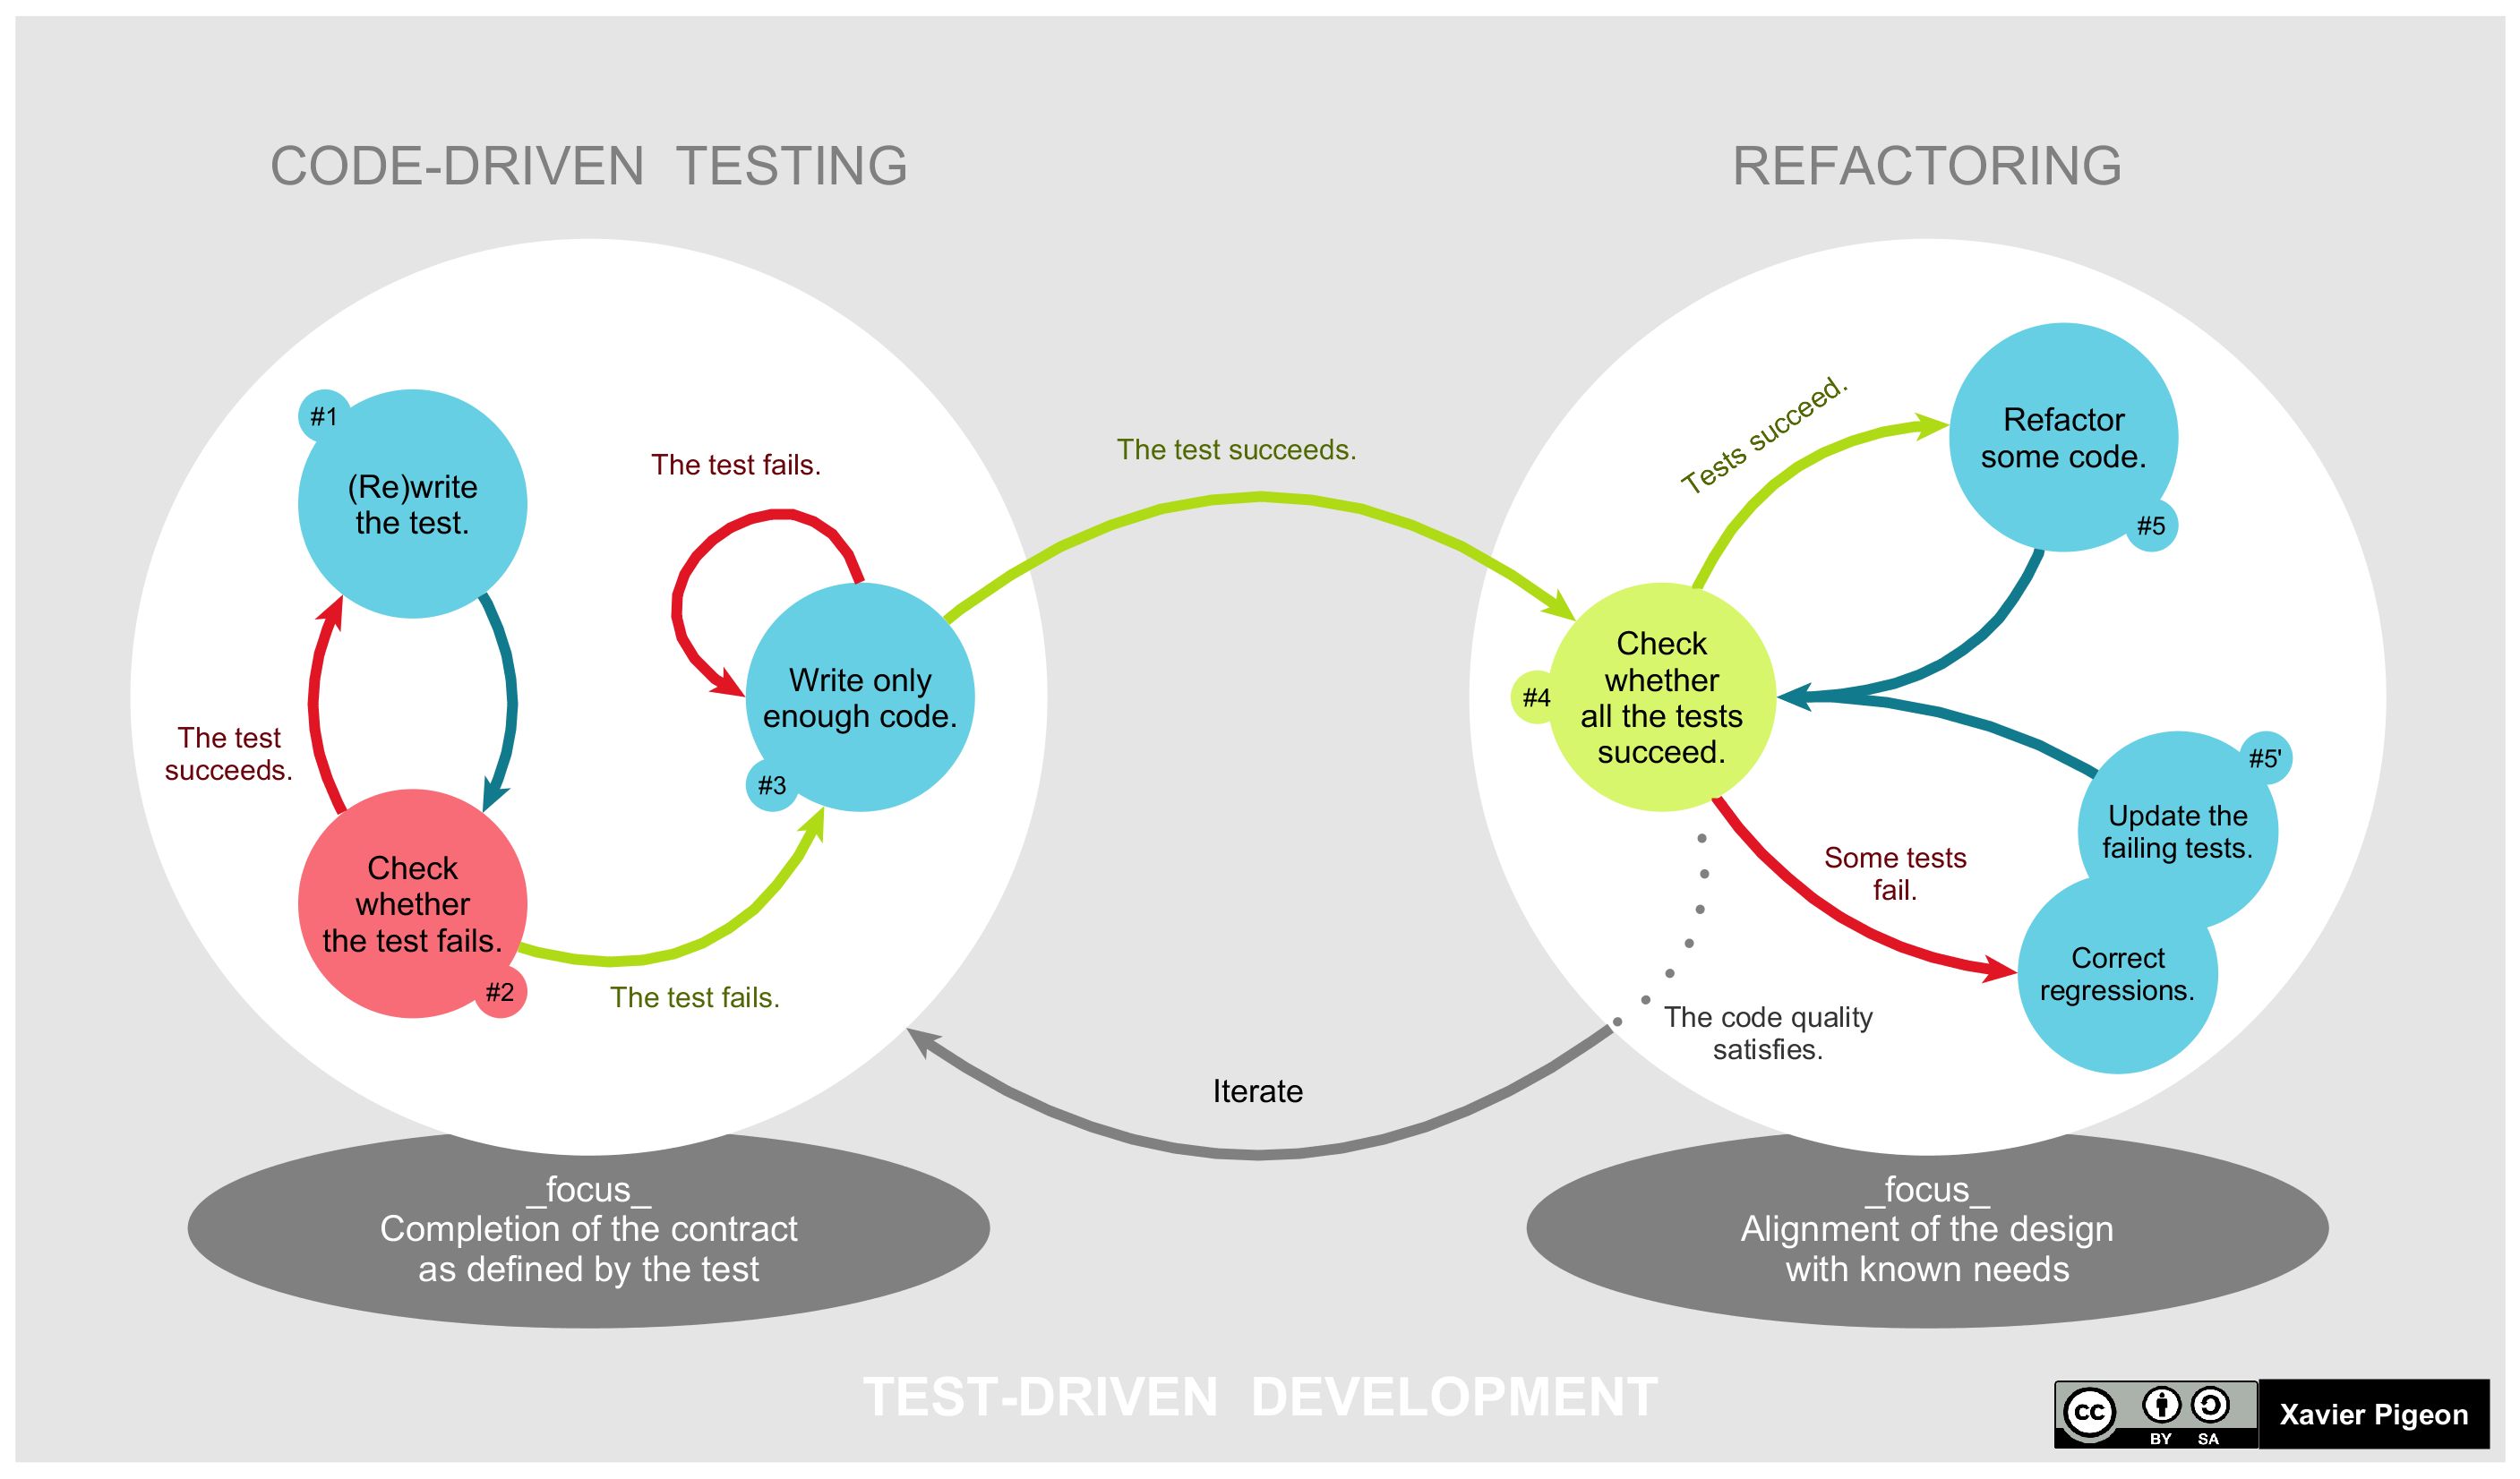
\includegraphics[width=\linewidth]{../assets/TDD_Global_Lifecycle.png}
    \caption{TDD Lifecycle \cite{Wikimedia:TDD}}
    \label{fig:tdd}
\end{figure}

TDD places an emphasis on first producing code that is minimally sufficient 
to pass the written tests. After which, code is refactored until it 
fulfils standard best practices such as readability, modularity, 
encapsulation etcetera. This appropriately prioritises functionality over 
readability, but still upholds written code to a high quality of design. 
This is especially so for this project as we prioritize correctness to 
ensure that we are providing meaningful results in our benchmarks.

Writing tests before implementation also helps during regression testing, to identify bugs 
when changes are made. This will not only improve code quality, but also make development 
more efficient. 


\subsection{Scrum and Kanban} Scrum is an agile project management framework that emphasises on 
flexibility and continuous improvement of software \cite{scrumguide}. 
It breaks down the development of a project 
into short iterations called sprints, which in our case are 2 weeks long. Meanwhile, Kanban is a 
another project management framework that share similar principles to Scrum and is often used 
in synergy with Scrum \cite{kanbanscrum}. Kanban focusses on visualising the workflow and 
limiting the number of features being worked on at any one time. This is done using a Kanban 
board, which is a visual representation of the tasks in the backlog, their current status, and 
the overall workflow. 
By controlling the number of features being worked on, 
it ensures that we complete features in a timely manner and do not run the risk of multitasking 
and causing delays. 

In this project, we use Kanban to manage our features and Scrums to manage development 
of said features. We use the Kanban board provided by Github to track all 
the features that we have planned for the project.
\begin{enumerate}
  \item Features are first added to the project backlog and then moved when the next sprint is
  planned. Features may be added to the backlog during development if need be, providing 
  flexibility while keeping the current sprint manageable. 
  \item At the start of each sprint, we plan the group of features to work on 
  for the next 2 weeks, and move them to the "To-do" column of the Kanban board. This column 
  is also known as the "Sprint Backlog".
  \item During the sprint, we move the features to the "Write Tests" column when we start writing 
  tests for the feature, based on the requirements.
  \item Once the tests are written, we start with the implementation and 
  move the feature to the "Implement" column. Throughout the implementation phase, we regularly 
  run tests to verify that the code is working as expected. We first focus on implementing 
  a minimally functioning feature, and testing for correctness. After which, features are 
  refactored to be more optimal if time allows for it. Tests may be refactored or added 
  when necessary to be consistent with the updated code or requirements.
  \item Once the feature is 
  fully tested and verified to be working, we move it to the "Done" column, indicating that 
  it is ready to be merged into our main branch. 
  \item At the end of the sprint, we review the features that were completed and ensure that 
  the project is on track with the timeline. We also plan the next sprint, repeating the cycle 
  again. Any additional features that were added to the backlog during implementation are 
  usually added during this planning phase to the next sprint.
\end{enumerate} 

To summarise, we use Kanban as a visualisation tool and to control the features in progress, Scrum 
is used to manage the development of these features in sprints. Finally, TDD is used to ensure 
that the code is correct and that the features meet the requirements. 

\section{Timeline}
We split the project into 3 main stages: research and learning, development of CDS94, and 
development of Stacking Sigmas. The two development stages also include benchmarking the 
respective compilers and anlaysing the data collected. We did not create a separate stage 
for the benchmarks because they were best done in parallel with the development of the
compilers.
In Table \ref{table:timetable_final}, we show the overall timeline of the project. In the "Goal" 
column, we indicate with a checkmark if the goal was achieved. Comments are provided in 
brackets where relevant. 

\begin{table}
  \centering
  \caption{Overall Project Plan}
  \begin{tabular}{p{0.2\linewidth}p{0.45\linewidth}p{0.25\linewidth}}
  \toprule
  \bf Sprint & \bf Main Task & \bf Goal \\ 
  \midrule
  T1 W1-2
  & Conduct necessary background reading and research.
  & Submit project specification. \checkmark
  \\\addlinespace[\rowheight]
  T1 W3-4
  & Understand the literature and extract requirements from the design of CDS94.
  & Must be capable of explaining CDS94 protocol to project supervisor. \checkmark
  \\\addlinespace[\rowheight]
  T1 W5-6
  & Familiarise with Rust and research libraries to use for implementation.
  & Finalise features to develop for CDS94 \checkmark
  \\\addlinespace[\rowheight]
  0 (T1 W7-8)
  & Begin implementation of CDS94.
  & Submit progress report. \checkmark
  \\\addlinespace[\rowheight]
  1 (T1 W9-10)
  & Implementing CDS94.
  & - (Completed goal in the next sprint early)
  \\\addlinespace[\rowheight]
  2 (Christmas Break)
  & Continue work on CDS94. 
  Start implement benchmarks. 
  Study and research \cite{StackingSigmas}.
  & \sout{Complete CDS94 }
  \\\addlinespace[\rowheight]
  3 (T2 W1-2)
  & Benchmark tests for CDS94 and collect data. Begin implementation of 
  Stacking Sigmas.
  & Complete benchmarks for CDS94. \checkmark
  \\\addlinespace[\rowheight]
  4 (T2 W3-4)
  & Implementing Stacking Sigmas. Update benchmark tests if necessary.
  & Complete implementation of Stacking Sigmas. (Delayed: 1 sprint)
  \\\addlinespace[\rowheight]
  5 (T2 W5-6)
  & Implementing Stacking Sigmas. 
  Benchmark Stacking Sigmas compiler and organise data collected for final presentation. 
  & Able to explain concepts in \cite{SpeedStacking} to project supervisor. (Delayed: 1 sprint)
  \\\addlinespace[\rowheight]
  6 (T2 W7-8)
  & Preparation for final presentation. Attempt basic implementation of Speed Stacking.
  & Present data to supervisor before presentation \checkmark
  \\\addlinespace[\rowheight]
  7 (T2 W9-10)
  & Continue with Speed Stacking.
  & Final Presentation. \checkmark
  \\\addlinespace[\rowheight]
  Easter Break
  & Write up of final report alongside exam revision.
  & Submit first draft of report for review (\checkmark).
  Complete Speed Stacking (No longer possible).
  \\\addlinespace[\rowheight]
  T3 W1-2
  & Final proof reading and editing of report.
  & Submit final report. \\
  \bottomrule
  \end{tabular}
  \label{table:timetable_final}
\end{table}


\paragraph{Research and Learning.} In the first stage of the project (6 weeks), time was dedicated 
to learning any background material and to study the literature. 
This was also the time when we familiarised ourselves with the programming language of choice: Rust. 
Tools and libraries that ended up being helpful to us in the project were also discovered during 
this period, through research and experimentation. It was imperative that we spent this time 
understanding the literature, as it would otherwise be difficult to implement the protocols accurately.
To ensure that we were ready to start development, we organised meetings with the 
project supervisor dedicated to clarifying details on the research material and to validate 
our understanding of the background material as a whole.  

\paragraph{Development.} The second and third stages (18 weeks) are similar in that they are 
dedicated to the development of the project. Yet, we decided to separate them into 2 stages as 
we anticipated that the time taken for the first stage (research) may be longer than 
we expect. In this scenario, we would be able to quickly re-prioritise and change the scope of 
the project if necessary. Fortunately, this was not the case and we were able to complete 
our initial objectives in time. 

This development phase is split into sprints: each of 2 weeks, except during the Christmas break 
where it was extended to 4 weeks. The CDS94 compiler was completed in the first 2 sprints, 
which surpassed our expectations. However, this did not include the implementation of the 
benchmarks and benchmarking CDS94. The benchmarks were completed over the next 2 sprints 
before work on 
the Stacking Sigmas compiler began. Unforunately, this took longer than expected due to the 
complexity of 
implementing the partially-binding vector commitment scheme. Furthermore, 
issues with the code were discovered during testing, which took an entire sprint to solve. 
During this period, we decided to not prioritise security testing on our compilers, and focus 
on correctness and collecting data from the benchmarks instead. In the end, development and 
benchmarking of Stacking Sigmas required 3 sprints, which is longer than expected but still within 
the time frame of the project. 

We also mentioned the possibility of implementing the 
Speed Stacking compiler \cite{SpeedStacking} in the project specification, and started work on 
it, but ultimately are not able to complete it in time for this report. That said, we still 
deem the project a success as we were able to complete the CDS94 and Stacking Sigmas compilers 
and collect insightful data from the benchmarks. 

\section{Project Management Tools}
We use Github to manage our entire project. Github is a web-based hosting service for version 
control using Git, and it also provides project management tools. Notably, it provides a 
Kanban board with "Github Projects" and sprint management with "Github Milestones". We manage 
features using the Kanban board, creating drafts when we are planning and converting these 
features into "Github Issues" when we are ready to start development. This automatically creates a 
Git branch for the feature, which we can work on and subsequently merge into our main branch 
when the feature is complete. 

\section{Risk Management}
Below we list the risks that we identified at the start of the project and how we mitigated
challenges that arose during development.
\begin{itemize}
  \item \textbf{Lack of experience.} We were not familiar with the Rust programming
  language or the background material initially and planned the project with this in mind. This 
  is why we dedicated the first 6 weeks to learning the language and the literature. Additionally,
  to prepare for the case that this phase would take longer than expected, we opted for an agile 
  development methodology to remain adaptive to changes in the project scope if necessary.
  \item \textbf{Unexpected challenges.} To prepare for unexpected delays in development, we 
  planned the project with a clear priority of the requirements: correctness firstly, then 
  usability and generality, followed by performance and security. This allowed us to focus on
  the most important aspects of the project first, and to prioritise the remaining features
  accordingly. Splitting the development of the two compilers into separate stages also allowed 
  for the possibility of changing the scope to focus on solely CDS94 if necessary. 
  \item \textbf{Machine Failure.} We used proper version control practices with the aid of 
  Git and Github to ensure that work can continue even if a machine fails. We also verified 
  that our programming tools were compatible with the university machines. This came in useful 
  when we had to switch to a different machine due to a hardware failure.
  \item \textbf{License Agreements.} The project relies on many existing libraries for 
  cryptographic primitives and other utilities. We ensured that the licenses of these libraries
  were compatible with our project. 
\end{itemize}

% clear description of the stages of the life cycle undertaken
% description of the use of appropriate tools to support development
\chapter{Design \& Implementation}\label{sec:design}
\section{Design}
\label{ch:design}

In this chapter, we describe the overall design of our solution to the problem identified in \Cref{ch:introduction}, building on work described in \Cref{ch:background}.

% clear description and rationale of research methods used

% \chapter{Implementation}\label{sec:implementation}
% \section{Implementation}
\label{ch:implementation}

In this chapter, we describe the implementation of the design we described in \Cref{ch:design}. You should \textbf{not} describe every line of code in your implementation. Instead, you should focus on the interesting aspects of the implementation: that is, the most challenging parts that would not be obvious to an average Computer Scientist. Include diagrams, short code snippets, etc. for illustration. 

\begin{enumerate}
    \item Translating protocol description from math and words into code.
    \begin{enumerate}
        \item Difficult because it is not a 1-1 mapping
        \item Need to think about efficiency and speed
        \item Even after that, you may make mistakes in the implementation and debugging becomes difficult because you have to conduct static analysis to understand what has gone wrong. For example, in 1 case I didn't realise that I unknowingly passed the same vector into two functions that were supposed to receive two different vectors. Really requires understanding ....
    \end{enumerate}
    \item Debugging 
    \begin{enumerate}
        \item Even when implementing code according to the description of the protocol; there are times when it still doesn't work.
        \item A unique way of debugging where static analysis is the only reasonable way
    \end{enumerate}
\end{enumerate}

\chapter{Evaluation}\label{sec:evaluation}
% Describe the approaches you have used to evaluate that the solution you have 
% designed in \Cref{ch:design} and executed in \Cref{ch:implementation} actually 
% solves the problem identified in \Cref{ch:introduction}.

% While you can discuss unit testing etc. you have carried here a little bit, 
% that is the minimum. You should present data here and discuss that. This might 
% include \emph{e.g.} performance data you have obtained from benchmarks, survey 
% results, or application telemetry / analytics. Tables and graphs displaying this 
% data are good.
In this chapter, we evaluate our implementation with respect to testing and
the results of our benchmarks. 

\section{Testing}\label{eval:testing}
We implement tests for all major components of our system based on our approach 
described in Section \ref{design:testing}. These tests have been scrutinised to ensure 
they test the expected behaviour of each component, especially those 
that are based on protocols from the literature. Readers who are interested can 
run these tests using the \texttt{cargo test} command, to verify that all tests pass. 
Using code coverage analysis, we also ensure that we do not miss any important test 
cases and that we are testing as much of our code and as many edge cases as possible.
We use the following command to generate a code coverage report:

\begin{lstlisting}[language=bash]
  cargo llvm-cov --open --ignore-filename-regex libs/stacksig-compiler/src/rot256
\end{lstlisting}

\begin{figure}[t]
  \centering
  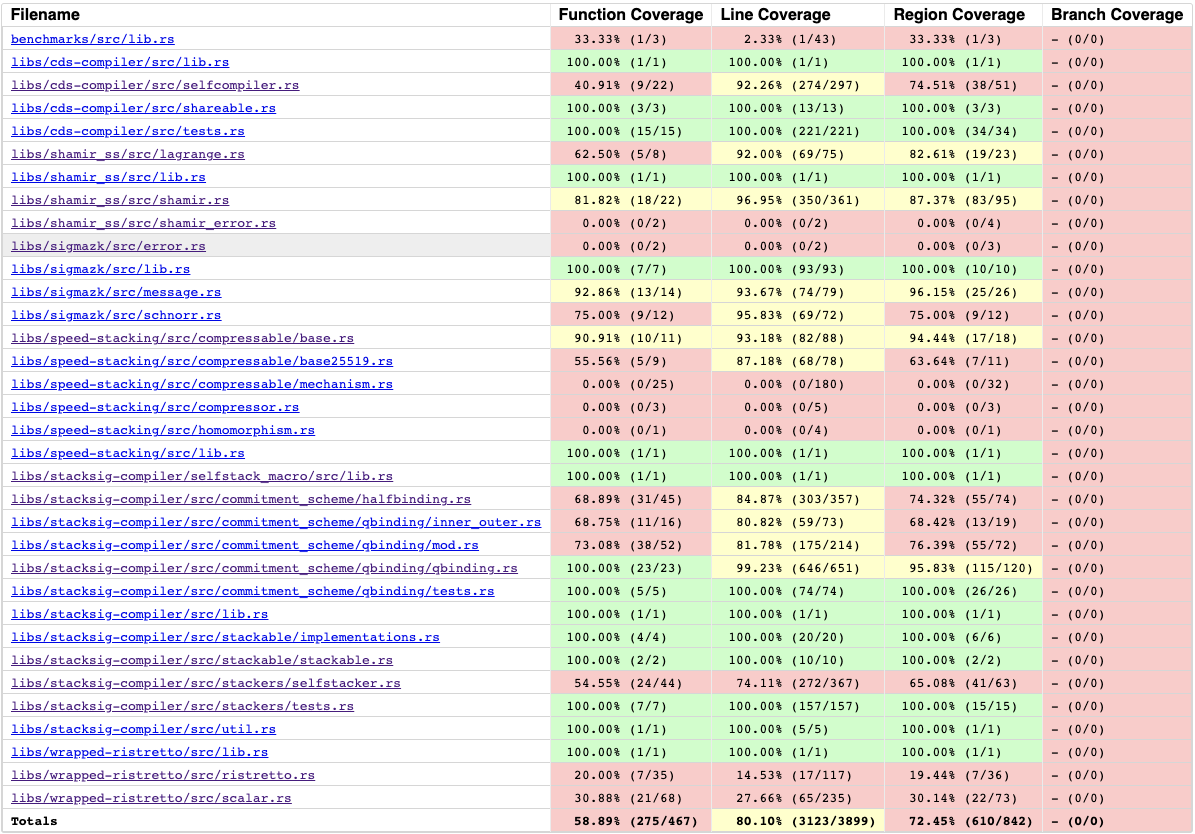
\includegraphics[width=\linewidth]{../assets/code-coverage.png}
  \caption{Code coverage of our project}
  \label{fig:coverage}
\end{figure}

The code coverage report produced by this command can be seen in Figure \ref{fig:coverage}. From this report, we observe that we have only 58.89\% function 
coverage (we only test 58.89\% of the functions in our project), 80.10\% line 
coverage, and 72.45\% region coverage\footnote{Regions are blocks of code with 
respect to the compiler -- these can be multiple lines of code with no control flow 
or a single line of code. These regions for Rust are determined by LLVM. \cite{llvm-cov-explain}}. These numbers may appear to be low, but upon closer inspection,
we observe the following:
\begin{enumerate}
  \item \textbf{Functions}: the majority of the functions that are not tested are either
  \begin{itemize}
    \item Getter and setter functions for classes (structs in Rust). These functions 
    simply return or set a value within the class, and are not tested as they are very simple. 
    \item or derived traits \cite{rust-book-derived-traits} in Rust. These are functions that are automatically generated according to "macros", which allow users to derive the implementation of specific interfaces for their classes automatically. These functions are not tested as they are automatically generated by the compiler. 
  \end{itemize}
  \item \textbf{Lines}: A portion of these lines include those for the Speed Stacking 
  compiler that we are still working on \cite{SpeedStacking}. These could not be 
  easily removed from the code coverage report, and affect the line coverage statistics.
  Additionally, many of these lines are automatically generated by the compiler from 
  derived traits. 
  \item \textbf{Regions}: While most regions are affected by the same reasons as functions and lines, it should be noted that there are some regions that should be 
  tested more thoroughly but are not. These regions are related to error producing 
  branches of code, which should be tested to ensure that our implementation handles 
  errors correctly. The bulk of these regions are located in our implementation of 
  Shamir's secret sharing scheme. However, due to the low priority, and time constraints 
  of this project, we have not been able to test these cases thoroughly.
\end{enumerate}

Aside from these areas, all the main requirements of our compilers and respective 
software components are tested thoroughly. While it is ideal to achieve higher 
than 80\% code coverage in all categories, we believe that code coverage useful in 
identifying potential areas of improvement for testing, but should not be used as the
sole metric for evaluating the quality of our tests. In fact, the code coverage report
was useful in highlighting that we previously did not implement a proper 
negative test for the CDS94 compiler as the block of code that returns false in 
the verification algorithm was not covered by any tests. This was subsequently fixed, 
improving the code coverage report marginally, but covering and important case 
for our compiler.

In summary, we assess that our quality and thoroughness of testing is sufficient 
for the scope of this project. However, we acknowledge that there is still room for
improvement in our testing, especially in the areas of error handling. 
\section{Benchmark Results}\label{eval:benchmarks}
In this section, we present the results of our benchmarks and discuss their 
implications. We have four benchmarks: two for the CDS94 compiler \cite{CDS94}, 
one for the Stacking Sigmas compiler \cite{StackingSigmas}, and one from Hall-Andersen's implementation \cite{MHAStackSig}. One of the two benchmarks for CDS94 compiler compares 
the growth of the key metrics against the number of active clauses (instead of the 
number of clauses). We will first present and discuss the results regarding the 
growth in communication size across all benchmarks. After which, we will discuss
the results for the growth in the computation time. In table \ref{tab:comm-size} and 
\ref{tab:comp-time}, we present the overall results of our benchmarks.

\begin{table}[H]
  \centering\caption{Communication Size Results (in bytes)} 
  \label{tab:comm-size}
  \begin{tabular}{rcc}
    \toprule
    \textbf{Clauses} & \textbf{CDS94} & \textbf{Stacking Sigmas} \\
    \midrule
    2 & 224 & - \\
    4 & 416 & 256 \\
    8 & 800 & 320 \\
    16 & 1568 & 384 \\
    32 & 3104 & 448 \\
    64 & 6176 & 512 \\
    128 & 12320 & 576 \\
    256 & 24608 & 640 \\
    512 & 49184 & 704 \\
    1024 & 98336 & 768 \\
    2048 & 196640 & 832 \\
    4096 & 393248 & 896 \\
    8192 & 786368 & 960 \\
    \bottomrule
  \end{tabular}
\end{table}

\begin{table}[H]
\centering
\caption{Computation Time Results (in milliseconds)}
\label{tab:comp-time}
\begin{tabular}{rccccc}
\toprule
\textbf{Clauses} & \textbf{StackSig Prover} & \textbf{CDS Prover} & \textbf{StackSig Verifier} & \textbf{CDS Verifier} & \textbf{Rot256} \\
\midrule
2 & 0.3 & 0.081124 & 0.3 & 0.10955 & 3.4760 \\
4 & 0.64893 & 0.19991 & 0.64233 & 0.22346 & 7 \\
8 & 1.8222 & 0.45870 & 1.3788 & 0.47586 & 10.9 \\
16 & 4.2626 & 0.98115 & 2.8526 & 0.97444 & 15.021 \\
32 & 9.3257 & 2.1472 & 5.9700 & 2.0985 & 20.069 \\
64 & 19.616 & 5.0377 & 11.705 & 4.9214 & 37 \\
128 & 40.584 & 13.105 & 24.474 & 12.696 & 37.131 \\
256 & 82.243 & 37.381 & 47.087 & 36.691 & 54.213 \\
512 & 165.70 & 120.33 & 93.798 & 118.92 & 85 \\
1024 & 334.63 & 422.50 & 190.63 & 419.73 & 145.33 \\
2048 & 671.82 & 1572.9 & 375.45 & 1583.5 & 257.25 \\
4096 & 1359.1 & 6110.2 & 742.17 & 6081.9 & 482.62 \\
8192 & 2685.4 & 24141 & 1477.9 & 23884 & 932.34 \\
\bottomrule
\end{tabular}
\end{table}

\paragraph{Running benchmarks.} To run our benchmarks on your own machine, you can 
use the \texttt{cargo bench} command. To run the benchmarks for a specific compiler,
you can use the \texttt{{-}{-}bench} flag. Below we provide an example of how to run
each benchmark available:
\begin{lstlisting}[language=bash]
  # run benchmark for CDS94 (as clauses increase)
  cargo bench --bench cds_benchmark 
  # run benchmark for CDS94 (as active clauses increase)
  cargo bench --bench cds_benchmark2 
  # run benchmark for Stacking Sigmas (as clauses increase)
  cargo bench --bench stacksig_benchmark 
  # run benchmark for Hall-Andersen's implementation (as clauses increase)
  cargo bench --bench rot256_benchmark
\end{lstlisting}

\subsection{Communication Size}\label{eval:comm}
We present two figures, Figure \ref{fig:cds_comm} and Figure \ref{fig:stacksig_comm},
for the CDS94 compiler and Stacking Sigmas compiler respectively. These figures 
show the growth in communication size for each compiler as the number of clauses
increases. Note that the $x$-axis of these figures is logarithmic. Therefore, a 
linear and logarthmic growth in communication size is represented by a quadratic and linear growth in the logarthmic scale respectively. 
\begin{figure}[h]
  \centering
  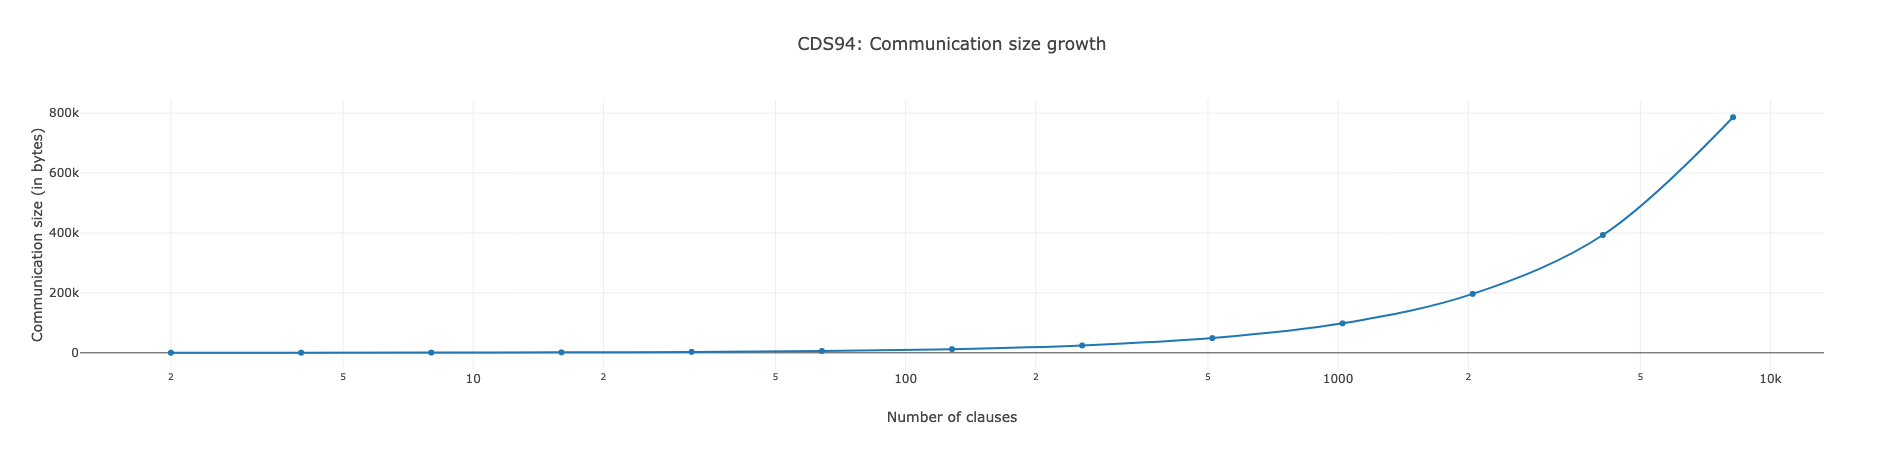
\includegraphics[width=\linewidth]{../assets/plots/cds_commsize.png}
  \caption{The growth in communication size for the CDS94 compiler. }
  \label{fig:cds_comm}  
\end{figure}

\begin{figure}[h]
  \centering
  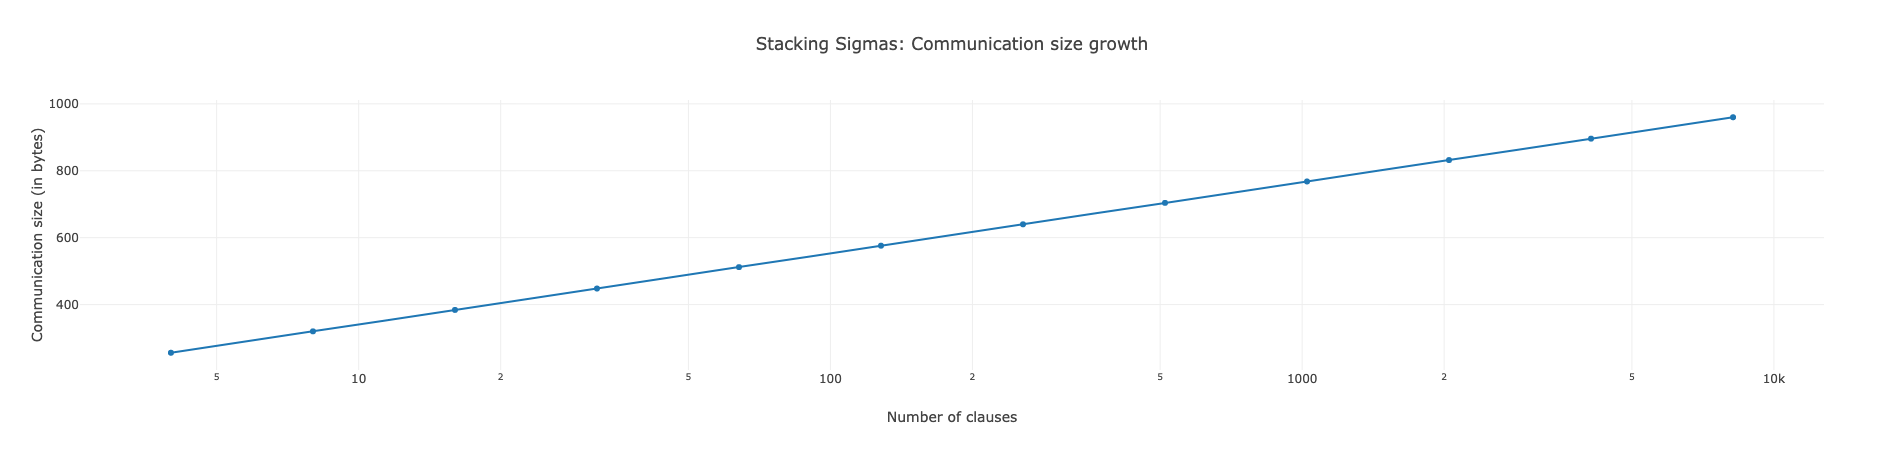
\includegraphics[width=\linewidth]{../assets/plots/ss_commsize.png}
  \caption{The growth in communication size for the Stacking Sigmas compiler. }
  \label{fig:stacksig_comm}
\end{figure}

In both cases, we point out that the communciation size growth is consistent with 
the theoretical proofs of the respective compilers. This further validates our
implementation of the compilers. The expected growth in communication size for
the CDS94 compiler is linear, which appears as a quadratic growth with a 
logarthmic scale. Meanwhile, the equivalent for the Stacking Sigmas compiler is
a logarthmic growth, which appears as a linear growth in the logarthmic scale. 

With an increasing number of active clauses, but a constant number of clauses, 
the communication size for the CDS94 compiler is not expected to change. This is
because the number of active clauses does not affect the number of elements in the 
vector of messages sent by the prover. This is supported by the results in Figure
\ref{fig:cds_comm2}. This figure shows that the communication size for 512 
clauses is constant at 53.28KB, regardless of the number of active clauses.

\begin{figure}[h]
  \centering
  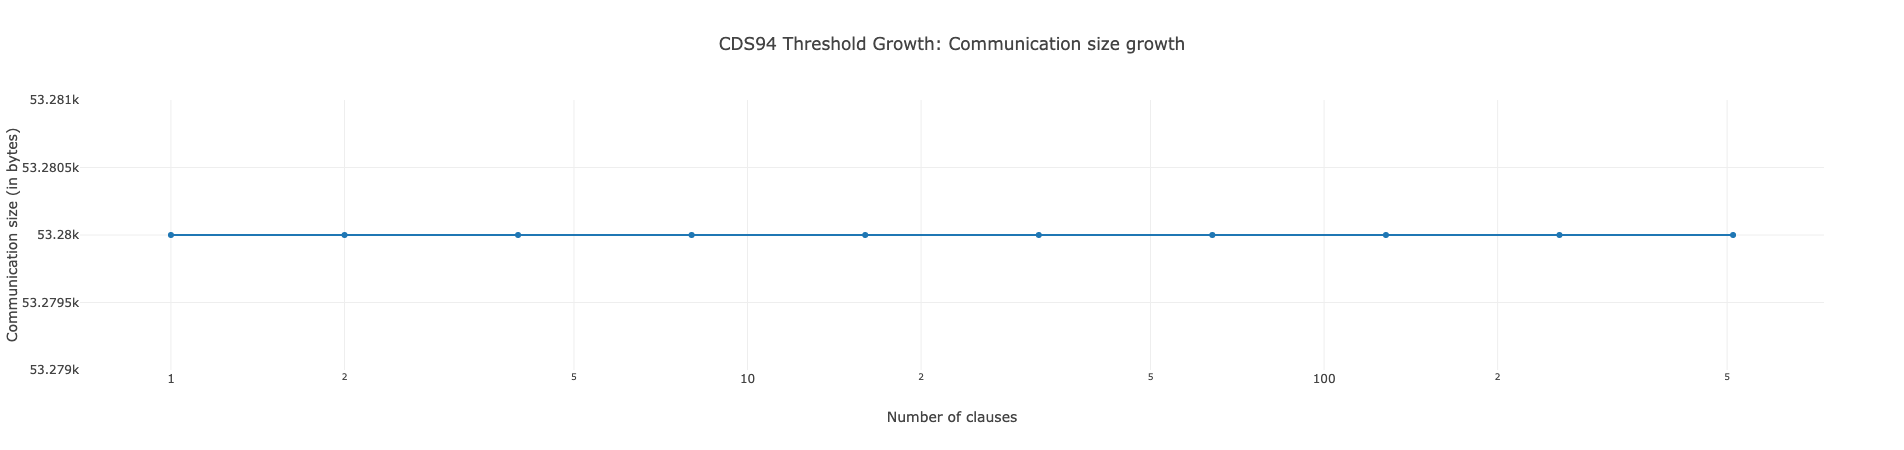
\includegraphics[width=\linewidth]{../assets/plots/cds2_threshold.png}
  \caption{The growth in communication size for the CDS94 compiler as the number of active clauses increases (total clauses = 512).}
  \label{fig:cds_comm2}
\end{figure}

We do not provide a similar figure for Hall-Andersen's implementation as the 
results are identical to Figure \ref{fig:stacksig_comm}. In conclusion, the 
observed growth in communication size is consistent with the theoretical
proofs of the respective compilers, further supporting the correctness of our
implementations, and also validating these proofs.

\subsection{Computation Time}\label{eval:time}
Firstly, we present the comparison between prover and verifier running 
time for each compiler. 

\paragraph{CDS94 Prover vs Verifier.} In Figure \ref{fig:cds_vs}, we compare the 
prover and 
verifier running time in our implementation of \cite{CDS94}. From the figure, 
we observe that the both running times are quadratic as 
the number of clauses increase. This is mainly because polynomial interpolation
using Lagrange is the bottleneck with a quadratic running time. This 
directly affects both the prover and verifier running times, as both the 
third round protocol and the verification algorithm uses this algorithm. 

\begin{figure}[H]
  \centering
  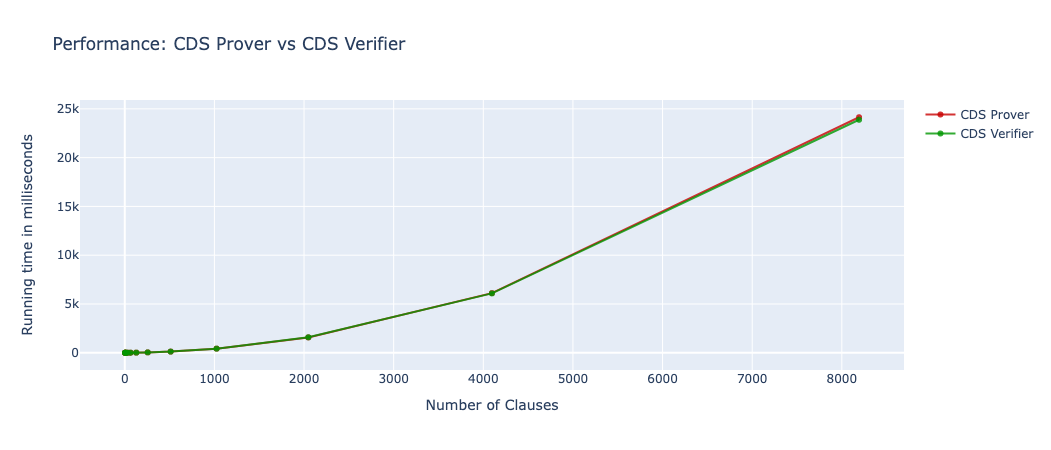
\includegraphics[width=\linewidth]{../assets/plots/cds_vs.png}
  \caption{A comparison of the prover and verifier running time of CDS94. }
  \label{fig:cds_vs}
\end{figure}

\begin{figure}[H]
  \centering
  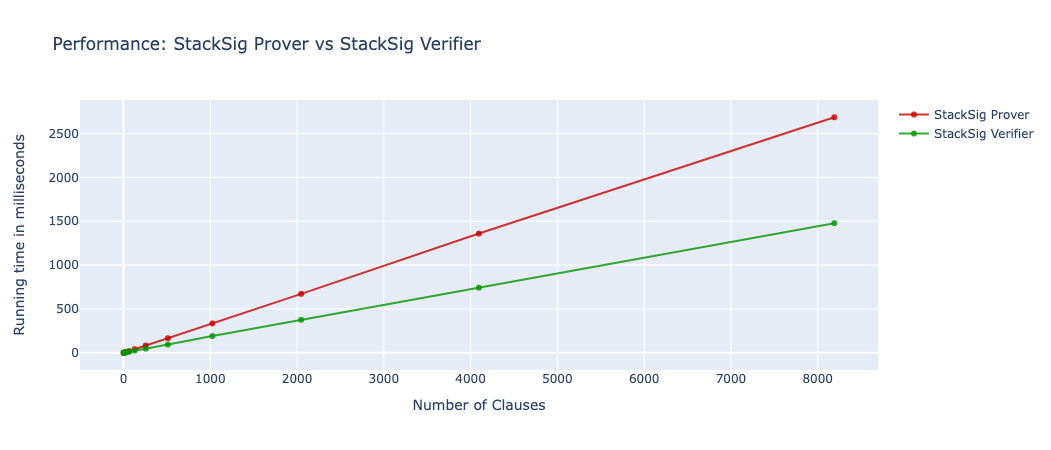
\includegraphics[width=\linewidth]{../assets/plots/ss_vs.png}
  \caption{A comparison of the prover and verifier running time of Stacking Sigmas.}
  \label{fig:stacksig_vs}
\end{figure}

\paragraph{Stacking Sigmas Prover vs Verifier.} In Figure \ref{fig:stacksig_vs}, we compare the prover and verifier running time
for the Stacking Sigmas compiler. This shows a linear growth in compuation time 
for both the prover and verifier, which is expected. The prover running time has 
a larger constant factor than the verifier running time. This is likely the case 
because the prover algorithms call the \textsf{Equiv} and \textsf{EquivCom} 
methods from the q-binding scheme, which are more computationally expensive than
the \textsf{Bind} method used in the verifier algorithm.

\paragraph{CDS94 vs Stacking Sigmas.} Next, we compare the prover algorithms of CDS94 and Stacking Sigmas. In Figure 
\ref{fig:provers_vs}, we see that up until 512 clauses, the CDS94 prover is more 
performant. However, due to the quadratic running time of the CDS94 prover, the 
Stacking Sigmas prover starts to outperform CDS94 after 512 clauses. 
Similarly in Figure \ref{fig:verifiers_vs}, where we compare the verifier algorithms 
across the two compilers, CDS94 is more performant when there are 256 or fewer clauses. 
 After which, Stacking Sigmas overtakes and takes less time to run. Note that both the 
$x$-axis and the $y$-axis are on the logarithmic scale. 

\begin{figure}[h]
  \centering
  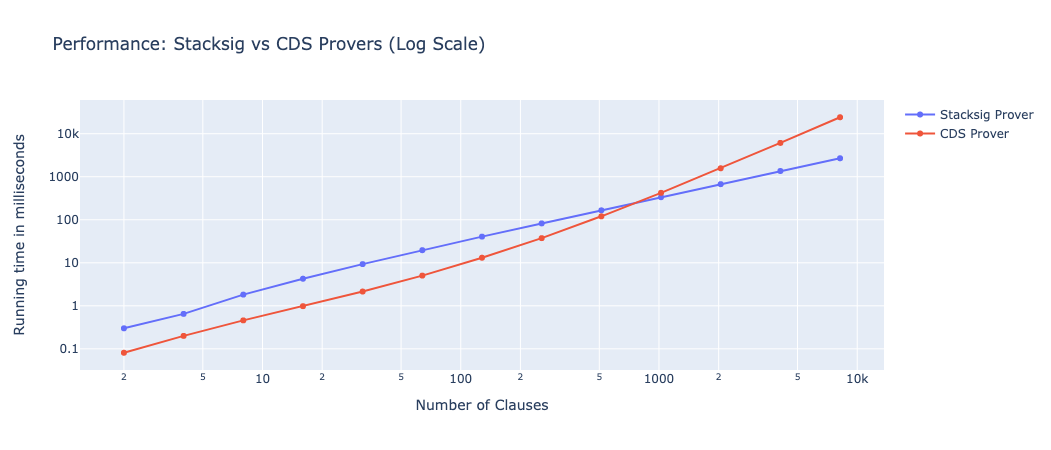
\includegraphics[width=0.9\linewidth]{../assets/plots/vs_provers.png}
  \caption{Comparison of CDS94 Prover and Stacking Sigmas Prover Algorithms.}
  \label{fig:provers_vs}
\end{figure}

\begin{figure}[H]
  \centering
  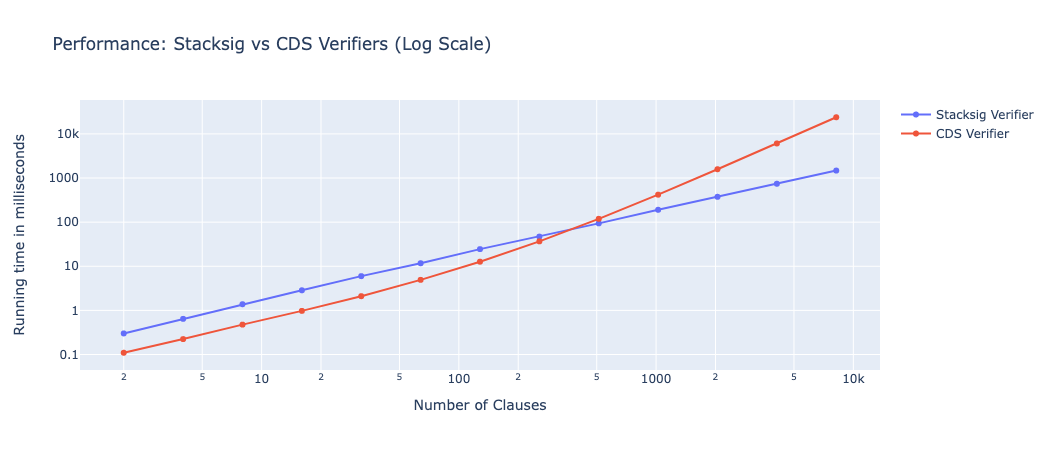
\includegraphics[width=\linewidth]{../assets/plots/vs_verifiers.png}
  \caption{Comparison of the Verifier algorithms of CDS94 and Stacking Sigmas.}
  \label{fig:verifiers_vs}
\end{figure}

These results indicate that if computation speed is the priority,
 it may be more appropriate to use Stacking Sigmas 
when the number of clauses is large (i.e. 512 or more), compared to an implementation of 
CDS94 that uses Lagrange's interpolation \cite{lagrange} with Shamir's secret sharing 
\cite{DBLP:journals/cacm/Shamir79}. That said, this only applies to 1-out-of-n 
disjunctive zero-knowledge, as k-out-of-n disjunctions are not supported by this 
implementation of Stacking Sigmas.

\paragraph{Total Running Time.} Extending this comparison, we now compare the total running time (prover and verifier)
of the three implementations. In Figure \ref{fig:3log}, we see that the total running time of the CDS94 compiler, the Stacking Sigmas compiler, and Mathias Hall-Andersen's 
implementation. We observe that the total running time of the CDS94 compiler and both 
impmlementations of Stacking Sigmas is similar to what we observer in 
Figures \ref{fig:provers_vs} and \ref{fig:verifiers_vs}. Comparing the two 
Stacking Sigmas implementations, we notice that the running time of Hall-Andersen's 
implementation is better starting from 128 clauses. As mentioned in Section 
\ref{design:qbinding}, this difference in performance is likely due to our 
decision to trade off performance for usability.


\begin{figure}[H]
  \centering
  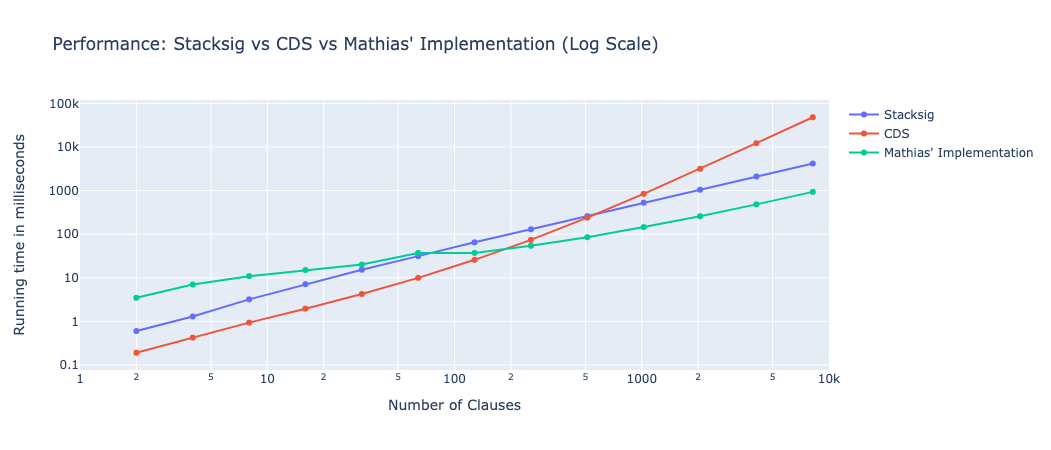
\includegraphics[width=0.9\linewidth]{../assets/plots/3log.png}
  \caption{Comparison of the total running time of the 3 compilers: \cite{CDS94}, 
  Stacking Sigmas \cite{StackingSigmas}, and
  Mathias Hall-Andersen's implementation \cite{MHAStackSig} of Stacking Sigmas.}
  \label{fig:3log}
\end{figure}

 

Our current implementation of the q-binding scheme leads to many calls to the 
\texttt{clone} function which duplicates data. The reason for this is mainly due 
to our lack of experience with Rust, and can be improved in future work. Furthermore, 
in Hall-Andersen's implementation, a protocol for every power of two number of 
clauses requires the instantiation of a new type. This means that 
a disjunction of 2 clauses, 4 clauses, 8 clauses, and so on, must use a different 
type. This is not ideal as it requires the developer to write a lot of boilerplate
code, and also results in code duplication. For this reason,
we believe that the trade off is sound as it allows for a more usable interface for 
developers and can be further improved. Moreover, this performance difference does 
not affect the correctness of the implemention or the goal of our benchmarks. 


\paragraph{CDS94 with increase in Active Clauses.} Finally, we plot the running time of the CDS94 prover and verifier as the number of
\textbf{active clauses} increase (every power of 2 from 1 to 512 active clauses). 
For this benchmark, we fix the total number of clauses to 512.

\begin{figure}[H]
  \centering
  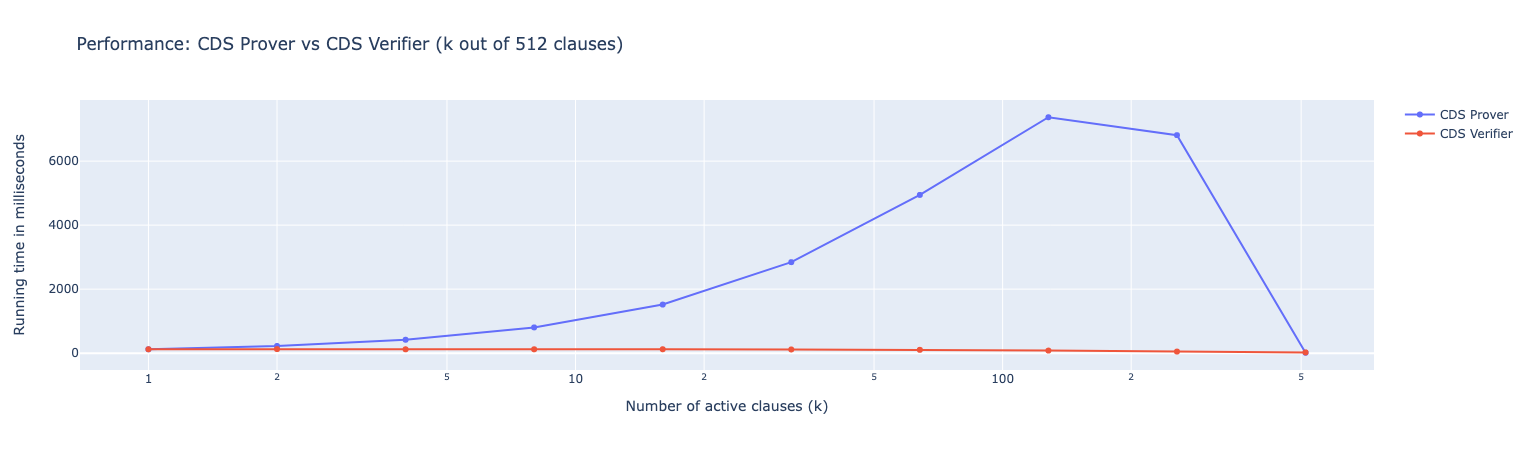
\includegraphics[width=\linewidth]{../assets/plots/cds_threshold.png}
  \caption{Comparison of prover and verifier algorithms as \textit{active clauses} increase. Note that the $x$-axis is on the logarithmic scale.}
  \label{fig:cds_threshold}
\end{figure}

In Figure \ref{fig:cds_threshold}, we see that the
prover running time peaks at 128 clauses, and drops abruptly at 512 clauses. Meanwhile, 
the verifier running time is constant as expected because the number of active 
clauses do not affect the verifier algorithm -- only the total number of clauses do.
The behaviour of the prover's running time can be directly attributed to 
our \textsf{Complete} algorithm (Definition \ref{def:sss-completion})
which we show in Listing \ref{lst:sss-completion}.

When completing the shares for the active clauses, we are required to interpolate 
at the point corresponding to the index of the active clause (this is the \texttt{x}
variable in the code listing). This interpolation 
uses the secret and the maximally unqualified set of shares to obtain the 
polynomial. As mentioned earlier, Lagrange's polynomial interpolation is an 
$O(n^2)$ algorithm, where $n$ is the number of points used to interpolate. 
Furthermore, the interpolation algorithm is called $k$ times where $k$ is the number of active 
clauses. This means that $n = \texttt{total clauses} - k + 1$. 

\begin{lstlisting}[language=rust, caption={Share Completion Algorithm},label={lst:sss-completion}]
  let remaining_shares = remaining_xs
      .iter()
      .map(|x| {
          let y = poly.interpolate(*x);
          Share { x: *x, y }
      })
      .collect();
\end{lstlisting}

Hence, the total running time of the \textsf{Complete} algorithm is $O(k \cdot n^2)$ (or
$g(k) = k \cdot (513 - k)^2$ in our case). By plotting function $g$ as a graph, we observe a 
direct correlation with what we observe in Figure \ref{fig:cds_threshold}. This is 
easy to see if we show this function as a table:

\begin{table}[H]
  \centering\caption{Active clauses \& $g(k)$}
  \vspace{0.5em}
  \begin{tabular}{lll}
    \toprule
    \textbf{Active Clauses} & \textbf{Threshold} & \textbf{$g$} \\
    \midrule
    1  & 512  & $262144$  \\
    2  & 511  & $522242$  \\
    4  & 509  & $1036324$  \\
    8  & 505  & $2040200$  \\
    16 & 497  & $3952144$ \\
    32 & 481  & $7403552$ \\
    64 & 449  & $12902464$ \\
    128 & 385 & $18972800$\\
    256 & 257 & $16908544$ \\
    512 & 1   & $512$ \\
    \bottomrule
  \end{tabular}
\end{table}

These results shed light on the effects of using Lagrange's polynomial interpolation algorithm 
with Shamir's secret sharing scheme. The CDS94 compiler \cite{CDS94} with Shamir's Secret Sharing 
and Lagrange's interpolation is most effective when the number of active clauses matches the 
total number of clauses. However, this is arguably an uninteresting case as it is no different to 
a \textit{conjunction} of clauses requiring the verifier to check every clause. In practice, we 
expect the number of active clauses to be in a smaller range. This indicates that Lagrange's 
interpolation algorithm is not the most ideal algorithm for Shamir's secret sharing scheme, 
as the running time increases cubically with the number of active clauses until it peaks 
at two powers of 2 below the total number of clauses.

\subsection{Summary of Results}
To summarise, we have firstly verified the proofs regarding the communication size of each 
compiler as the results here are consistent with the results in the literature 
\cite{CDS94,StackingSigmas}. 

Next, we have revealed important insights into the performance 
of the CDS94 and Stacking Sigmas compiler. It is clear that our implementation of the 
CDS94 compiler is significantly faster than the Stacking Sigmas compiler when the number of 
clauses are small. That said, the Stacking Sigmas compiler has a communication size that 
grows logarithmically with the number of clauses, while the CDS94 compiler's communication
size grows linearly. Hence, the trade off has to be made between the need for a smaller 
communication size and the need for a faster computation time. 

In general, we believe that 
the Stacking Sigmas compiler is more suitable in any use case where a 1-out-of-n 
disjunctive proof is suitable. This is primarily because of the large savings 
in communication size (kilobytes of data) and the small increase in computation time 
(a few milliseconds) of using it when the number of clauses are small. When the number of 
clauses increase, CDS94 performs worse and the performance degradation is far more significant 
because of the large number of clauses. For use cases where a k-out-of-n threshold proof is 
required, the CDS94 compiler has to be used. Further improvements could be made to 
our implementation of CDS94 to further reduce computation time and improve performance 
as the number of active clauses or total number of claues increase. This will be interesting 
to explore in future work. 


% description of outcome of research (results)
% critical appraisal of project indicating rationale for methods used, lessons learnt
% during the project, evaluation of the outcome (review plan, and deviations)

\chapter{Conclusions}\label{sec:conclusions}
Overall, we accomplished our goals of firstly implementing the CDS94 \cite{CDS94} and Stacking 
Sigmas \cite{StackingSigmas} compiler, and secondly benchmarking their performance. Through our 
work, we have shown that Stacking Sigmas outperforms CDS94 by providing significant savings in 
the communication size of the proof, especially as the number of clauses increases. 
Furthermore, while CDS94 is faster than Stacking Sigmas when the number of clauses is small,
we show that the difference in speed is negligible because the number of clauses is small. 
When the number of clauses increases, the difference in speed is more significant and CDS94 
performs worse than Stacking Sigmas in this case. Moreover, we also reveal that the bottleneck of the CDS94 compiler is the secret sharing scheme,
and highlight how the choice of this scheme and its implementation has a significant impact on the performance
of the compiler. This is all while we uphold our goal of keeping the implementation of the compiler
easily usable and extensible, in order to lay a good foundation for future work in this area. 

Additionally, there were many useful lessons that we learnt throughout the project. Firstly, we 
learnt the importance of proper project management and planning for a successful project. The 
risk management plan that we created at the start of the project helped us to identify potential
risks and to mitigate them. This allowed us to focus on the project and avoid any distractions
that could have hindered our progress significantly. Secondly, we realised the importance 
and convenience of good testing practices. Because of our testing practices, we were able to
identify and fix bugs early, accelerating our progress. Lastly, we were able to learn more about 
the inner workings of zero-knowledge proofs and other cryptographic concepts. Work in this field 
is often theoretical, and it is interesting to see how these concepts can be implemented in practice.

\section{Future work}\label{sec:futurework}
Aside from addressing the immediate limitations of this project (Section \ref{sec:limitations}), there are many directions in which we can extend the work in this project. Below we include separate paragraphs for each possible extension of our work. 

\paragraph{Benchmarks.} Firstly, we suggest an extension to the benchmarks that we provide in our work. Currently, across the different benchmarks, there is too much boilerplate code resulting in repeated sections of code. Additionally, there are parts of the process that are done manually. These include the collection of benchmark timings into CSV (comma-separated values) for further data analysis and the creation of mock data for the benchmarks. An implementation of a benchmarking framework that provides a convenient testing interface for various compilers would be very helpful in this case. This framework should have features to produce mock data and extract raw metrics from our benchmarks into CSV automatically. This will help to enhance the benchmarking process, accelerating research time and reducing errors in data collection. Currently, there are means of generating CSV files containing raw data using the \texttt{criterion} library \cite{criterion}. However, this functionality the library provides is in the midst of being deprecated and replaced by other tools. A good start would be to look into the \texttt{cargo-criterion} tool \cite{criterion} which outputs data from benchmarks into a \texttt{json} file. Unfortunately, there was insufficient time to prioritise this within this project. 

\paragraph{Speed Stacking.} Secondly, our work on the 
Speed Stacking compiler \cite{SpeedStacking} is not complete. We have implemented the base $\Sigma$-protocol of our choice (Compressed $\Sigma$-protocols \cite{attema}) but have yet to implement the compiler proposed in the paper \cite{SpeedStacking}. Given more time, we would have wanted to include this in our contributions to this project and present the results of the benchmarks conducted on it. The current challenge with this task is designing the compiler in \cite{SpeedStacking}, which is a multi-round compiler (with more than 3 rounds), to work with our interfaces. Once this is implemented, it will become possible to benchmark this compiler with other base protocols such as interactive oracle proofs \cite{iops}. 

\paragraph{Stacking Sigmas.} Next, our implementation of Stacking Sigmas is the Self-Stacking 
implementation, where we use the same $\Sigma$-protocol for each clause. We can also implement
the Cross-Stacking compiler \cite{StackingSigmas}, which is compatible with different $\Sigma$-protocols for each clause.
This would allow us to compare the performance of the compiler when using different $\Sigma$-protocols, 
and possibly test how the choice of $\Sigma$-protocols affects the performance of the compiler. 

An alternative is to explore Goel {\em et al.}'s idea for a $k$-out-of-$l$ compiler (Section 9 of \cite{StackingSigmas}).
This idea relies on the parallel execution of $k$ 1-out-of-$l$ proofs together with a family of hash functions to 
ensure that the verifier can check that each execution is for a unique clause. 

\paragraph{CDS94.} Similar to Stacking Sigmas, we can also explore the idea of compiling different $\Sigma$-protocols with the CDS94 compiler \cite{CDS94}. This may help to reveal insights into the relationship between the compiled protocols and the resulting disjunctive proof. 

Congruently, an idea that is more closely related to this project is to explore using better secret-sharing schemes or a more efficient implementation of Shamir's secret-sharing scheme with our CDS94 compiler. This would allow us to compare the performance of
the compiler when using different secret sharing schemes, and test how the choice of secret sharing scheme affects the performance of the compiler. Combining the previous two suggestions, it would then be interesting to identify if there exists an ideal secret-sharing scheme for the CDS94 compiler for both cross-compiling (different types of $\Sigma$-protocols) and self-compiling.

\paragraph{Multi-threading.} Lastly, we hypothesise that both the Stacking Sigmas and CDS94 compiler can be further improved with multi-threading. Both compilers rely on executing the various rounds of the nested protocols (the ones that are being compiled). The inputs to these executions do not depend on each other and can be executed in parallel without affecting the resulting proof. It would be interesting to study to what extent multi-threading can improve the performance of our compilers and whether it becomes feasible to be used for real-world applications. \\ 

To summarise, our work in this project has revealed various paths for further development of disjunctive zero-knowledge compilers. We hope that our efforts will help to accelerate future work in this area and drive the eventual use of these compilers in production.

\section*{Acknowledgements}
\label{sec:acknowledgements}
We would like to thank our supervisor, Nicholas Spooner, for his invaluable guidance and support throughout the project.


\printbibliography

\appendix
\addtocontents{toc}{\protect\setcounter{tocdepth}{1}}% This turns off subsections
\chapter{Code Snippets}\label{ch:code-snippets}
Input types are presented within the brackets of each method and 
output types are presented after the \texttt{->} symbol. For example, in section \ref{code:SigmaProtocol}, 
the \texttt{first} method has the input:

\texttt{statement: \&Self::Statement, witness: \&Self::Witness, prover\_rng: \&mut R}

and the output: 

\texttt{(Self::State, Self::MessageA)}

\section{\texttt{SigmaProtocol Interface}}
\label{code:SigmaProtocol}
\begin{lstlisting}[language=rust]
  fn first<R: CryptoRngCore>(
      statement: &Self::Statement,
      witness: &Self::Witness,
      prover_rng: &mut R,
  ) -> (Self::State, Self::MessageA)
  where
      Self: Sized;

  fn second<R: CryptoRngCore>(verifier_rng: &mut R) -> Self::Challenge
  where
      Self: Sized;

  fn third<R: CryptoRngCore>(
      statement: &Self::Statement,
      state: Self::State,
      witness: &Self::Witness,
      challenge: &Self::Challenge,
      prover_rng: &mut R,
  ) -> Self::MessageZ
  where
      Self: Sized;

  fn verify(
      statement: &Self::Statement,
      a: &Self::MessageA,
      c: &Self::Challenge,
      z: &Self::MessageZ,
  ) -> bool
  where
      Self: Sized;
\end{lstlisting}

\section{\texttt{HVzk} \& \texttt{EHVzk} Interface}
\label{code:hvzk}

\begin{lstlisting}[language=rust]
  /// Honest-Verifier Zero Knowledge
  pub trait HVzk: SigmaProtocol {
      fn simulate(
          statement: &Self::Statement,
      ) -> (Self::MessageA, Self::Challenge, Self::MessageZ);
  }

  /// Extended Honest-Verifier Zero Knowledge
  pub trait EHVzk: SigmaProtocol {
      fn simulate(
          statement: &Self::Statement,
          challenge: &Self::Challenge,
          z: &Self::MessageZ,
      ) -> Self::MessageA;
  }
\end{lstlisting}

\section{Schnorr's Protocol}\label{code:schnorr}
\lstinputlisting[language=rust]{code/schnorr.txt}

\section{CDS94 Compiler: \texttt{SelfCompiler}}\label{code:cds}
\lstinputlisting[language=rust]{code/cds.txt}

\section{Stacking Sigmas Compiler: \texttt{SelfStacker}}\label{code:stacksig}
\lstinputlisting[language=rust]{code/stacksig.txt}

\section{Test Example: CDS94 Tests}\label{code:cds-tests}
\lstinputlisting[language=rust]{code/cds_tests.txt}

\chapter{Progress Report}
\section{Introduction}

Zero-Knowledge proofs \cite{GMR85} are protocols that allow a prover to convince a verifier that an NP statement is true, while revealing no additional information except the validity of their assertion. Early research proved that all languages in NP have zero-knowledge proof systems \cite{DBLP:conf/focs/GoldreichMW86}, and recent results have provided more efficient zero-knowledge proofs that are being used in practice. 

In many cases, it is desirable to have a zero-knowledge proof for a disjunctive statement, which is an NP statement with a set of clauses that are connected with logical ORs. Disjunctive statements have very useful properties that occur commonly in practice, such as proving ones membership to a particular group, or showing the existence of a bug in a verifier's code base \cite{StackedGF}. Zero-knowledge becomes an important property in cases where revealing the exact clause (or clauses) that is true may reveal private information about the prover, such as their identity. A long line of research has focussed on how $n$ zero-knowledge proofs, each for one statement, can be composed into a new zero-knowledge proof of the disjunction of these statements. 

In their 1994 paper, Cramer, Damg{\aa}rd, and Schoenmakers \cite{CDS94} provide a generic compiler to compose 3-round public coin proofs of knowledge, or more succinctly (and more popularly) known as $\Sigma$-protocols. %perhaps discuss more
More recently, Goel {\em et al.} \cite{StackingSigmas} improved on this further, providing a generic compiler for a large class of $\Sigma$-protocols and also reducing the size of the resulting proof. 

While extensive research has been conducted, there is a lack of notable real-world implementations of these results
\footnote{It should be noted that Hall-Andersen \cite{MHAStackSig} has provided a benchmark of applying the compiler in \cite{StackingSigmas} to Schnorr's discrete log protocol \cite{Schnorr}.}. This project seeks to build upon their work by implementing the compilers described in \cite{CDS94} and \cite{StackingSigmas}. Once implemented, we aim to provide a benchmark for both protocols to explore and measure how they differ. This will hopefully provide some valuable insights as to how these designs perform in practice, which may in turn lead to further improvements in the future that may have a broad impact on existing and upcoming cryptographic systems that rely on such a use case. 

\subsection{Related work}
\label{sec:related_work}
As part of their work in \cite{StackingSigmas}, Hall-Andersen provides an implementation of the Stacking Sigmas (SS) compiler \cite{MHAStackSig}. In this implementation, they apply the SS compiler to Schnorr over Ristretto25519 to obtain efficient ring signatures from discrete log and random oracles. 

% Stacked Garbling implementation
\section{Background}
\label{sec:background}

\subsection{Disjunctive Zero-Knowledge}

\begin{definition}[NP Relations]
Let $R \subseteq \{0,1\}^* \times \{0,1\}^*$ be a binary relation. Then $w(x) = \{w \mid (x,w) \in R\}$ and $L_R = \{x \mid \exists w, (x,w) \in R\}$. If $(x,w) \in R$, we say that $w$ is a witness for $x$. $R$ is an NP-relation if it fulfils the following two properties:
\begin{enumerate}
    \item \textbf{Polynomially bounded.} We say that $R$ is \textit{polynomially bounded} if there exists a polynomial $p$ such that $|w| \le p(|x|), \forall (x,w) \in R$. 
    \item \textbf{Polynomial-time verification.} There exists a polynomial-time algorithm for deciding membership in $R$. Consequently, $L_R \in NP$. 
\end{enumerate}

Throughout this document, we will use $\mathcal R$ to refer to a binary NP-relation.
\end{definition}

\begin{definition}[Zero-Knowledge]
A proof or argument system $(P,V)$ is zero-knowledge over $\mathcal R$ if there exists a \textit{probabilistic polynomial time} (PPT) simulator $\mathcal S$, such that for all $(x,w) \in R$, the distribution of the output $\mathcal S(x)$ of the simulator is indistinguishable from $\ViewPV$, which denotes the distribution over transcripts generated by the interaction of $P$ and $V$ within the proof or argument system.
\end{definition}

Intuitively, this means that $V$ should not learn anything from the transcripts  with $P$ that they cannot already learn on their own by running the simulator $\mathcal S$; they learn nothing new.

\begin{definition}[Disjunctive Zero-Knowledge]
Given a sequence of statements $(x_1,x_2,\ldots, x_l)$, a \textit{disjunctive zero-knowledge proof} is a protocol to prove in zero-knowledge that $x_1 \in \mathcal L_1 \lor x_2 \in \mathcal L_2 \lor \ldots \lor x_l \in \mathcal L_l$, for NP languages $\mathcal L_i$. We term clauses for which the prover has a witness for as \textit{active} clauses. 
\end{definition}

\begin{definition}[Honest-Verifier Zero-Knowledge]
A proof system is \textit{honest-verifier zero-knowledge} if it only requires that $\mathcal S$ is an efficient simulator for honest (non-malicious) probabilistic polynomial time verifier strategies $V$. If $V$ is malicious then the distribution of the output $\mathcal S(x)$ will no longer be indistinguishable from $\ViewPV$ for such proof systems. 
\end{definition}

\subsection{$\Sigma$-protocols}
\begin{definition}[$\Sigma$-Protocol]
Let $\mathcal R$ be an NP relation. A $\Sigma$-protocol $\Pi = (A, Z, \phi)$ for $\mathcal R$ is a 3-round protocol between a prover algorithm $P$ and a verifier algorithm $V$. Conversations between $P$ and $V$ are ordered triples of the form $(a,c,z)$, and are known as \textit{transcripts}. The protocol consists of a tuple of probabilistic polynomial time algorithms $(A, Z, \phi)$ with the following interfaces:
\begin{itemize}
    \item $a \leftarrow A(x,w; r^p)$ : Given statement $x$, witness $w \in w(x)$, and prover randomness $r^p$ as input; output the first message $a$ that $P$ sends to $V$ in the first round. 
    \item $c \samplefrom \{0,1\}^\kappa$: $V$ samples a random challenge $c$ and sends it to $P$ in the second round. 
    \item $z \leftarrow Z(x,w,c; r^p)$: Given $x$, $w$, $c$, and $r^p$ as input; output the message $z$ that $P$ sends to $V$ in the third round.
    \item $b \leftarrow \phi(x,a,c,z)$: Given $x$, and the messages in the transcript, output a bit $b \in \{0,1\}$. This algorithm is executed by $V$, and $V$ accepts if $b = 1$.
\end{itemize}
A $\Sigma$-protocol has the following properties:
\begin{enumerate}
    \item \textbf{Completeness.} $\Pi$ is complete if for any $x$, $w \in w(x)$, and any prover randomness $r^p \samplefrom \{0,1\}^\lambda$, the following holds:
    \begin{gather*}
        Pr\left[\phi(x,a,c,z) = 1 \st a \leftarrow A(x,w;r^p); c\samplefrom \{0,1\}^\kappa; z \rightarrow Z(x,w,c;r^p)\right] = 1
    \end{gather*}
    \item \textbf{Special Soundness.} $\Pi$ is said to have special soundness if  there exists a PPT extractor $\mathcal E$, such that given any two transcripts $(a,c,z)$ and $(a,c',z')$ for statement $x$, where $c \ne c'$ and $\phi(x,a,c,z) = \phi(x,a,c',z') = 1$, an element of $w(x)$ can be computed by $\mathcal E$.
    \item \textbf{Special Honest-Verifier Zero-Knowledge.} $\Pi$ is SHVZK if there exists a PPT simulator $\mathcal S$, such that for any $x$, $w$, $(x,w) \in \mathcal R$, the distribution over the output $\mathcal S(x, c^*)$ is indistinguishable from the distribution over transcripts produced by the interaction between $V$ and $P$ when the challenge is $c^*$.
    \begin{multline*}
        \{(a, z) \mid c^* \samplefrom \{0,1\}^\kappa; (a,z) \leftarrow \mathcal S(1^\lambda,x,c^*)\} 
        \approx_{c^*} \\
        \{(a,z) \mid r^p \samplefrom \{0,1\}^\lambda; a \leftarrow A(x,w;r^p); c^* \samplefrom \{0,1\}^\kappa; z \leftarrow Z(x,w,c^*;r^p)\}
    \end{multline*}
    
\end{enumerate}


\end{definition}



Explain transcripts, witness indistinguishable and WH protocols. Explain HVZK and SHVZK?

\subsection{Schnorr's Identification Protocol}
There are two parties in an \textit{identification scheme}, the prover $P$ and the verifier $V$, and the objective of the protocol is for the prover to convince the verifier that they are who they claim to be. More precisely, $V$ is convinced that $P$ knows the private key that corresponds to the public key of $P$. A familiar example is the standard protocol of password authentication.

Schnorr's protocol \cite{Schnorr} is an identification scheme where $P$ proves knowledge of the discrete log $x$ of a group element $H \in \G$, where $H = x \cdot G$ for some generator $G \in \G$. $(\G, +)$ is a finite abelian group with $+$ as the binary operator\footnote{We have chosen to define $\G$ with the $+$ operator because our implementation uses elliptic curves which are finite abelian groups over addition. The discrete log can be defined equivalently with multiplication like so: $h = g^x$}. The protocol relies on the assumption that finding $x$ given only $H$ and $G$ is computationally difficult -- this is not always the case. The hardness of finding the discrete log depends on the choice of group $\G$ (cite some resource or elaborate). Conversely, proving that $H = x \cdot G$ given $x$ and $G$ can be computed efficiently. 

In our implementation, we plan to use the Ristretto group \cite{ristretto_web}: a construction of a prime order group from a family of elliptic curves known as Edwards curves \cite{Edwards2007}. 

\begin{definition}[Schnorr's Protocol \cite{Schnorr}]
Let $\G = E(\F_q)$, where $E$ is an elliptic curve over the finite field $\F_q$. Suppose that both the prover $P$ and verifier $V$ agree on $E$ and $\F_q$, then let $H \in E(\F_q)$ be the public key that corresponds to the private key $x$ such that $H = x \cdot G$. The prover convinces the verifier that they have knowledge of the private key by doing the following:

\begin{enumerate}
    \item $P$ generates random $r \in \F_q$, and computes the point $U = r \cdot G$. $P$ sends the point $U$ to $V$.
    \item $V$ computes a random $c \in \F_q$, and sends $c$ to the $P$.
    \item $P$ computes $z = (r + c \cdot x_P) \mod n$, and sends $z$ to the $V$.
    \item $V$ checks that $z \cdot G = U + c \cdot H$.
\end{enumerate} 

Evaluating the final equation, we can easily see that $V$ accepts if and only if $x = x_P$. 

\begin{equation*}
    z \cdot G = U + c \cdot H \iff
    r \cdot G + c \cdot x_P \cdot G  = r \cdot G + c \cdot x \cdot G \iff
    x  =  x_P
\end{equation*}
\end{definition}


\textbf{A simulator for Schnorr's protocol.} We construct a simulator for Schnorr's protocol by running it "in reverse":

\begin{center}
    \begin{problem}[]{Let our simulator be $S(H)$}
    $z \randselect \F_q$ ($\randselect$ = select randomly from)
    
    $c \randselect \F_q$
    
    $U = z \cdot G - c \cdot H$
    \tcblower
    \textbf{output} $(U,c,z)$
    \end{problem}
\end{center}

Since $z$ and $c$ are both chosen randomly, the resulting $U$ is also random, and our output will have the same distribution as the distribution over transcripts in an actual interaction.

\subsection{Shamir's Secret Sharing Scheme}
A \textit{secret sharing scheme} is a method of distributing a secret $s$ to $n$ participants in a way that no one participant has intelligible information about the secret. This is achieved by splitting up $s$ into \textit{shares}, distributing one share to each participant in a way that a subset of participants can reconstruct $s$. Subsets that can reconstruct the secret are called \textit{qualified sets}. For \textit{perfect} secret sharing schemes, like Shamir's, participants in the complement \textit{non-qualified} sets cannot obtain any information about the secret.

Shamir's secret sharing scheme \cite{DBLP:journals/cacm/Shamir79} is also what is known as a \textit{threshold sharing scheme}. These are schemes that produce  qualified sets of size $d$. Any $d$ out of $n$ participants can reconstruct the secret; with $d-1$ shares and less, no  information about the secret can be obtained. 

\subsection{CDS94 Compiler}


In our implementation, we will use Schnorr's discrete log protocol over Ristretto25519 and Shamir's secret sharing scheme to demonstrate the compilation of $\Sigma$-protocol into a $\Sigma$-protocol for the disjunction of $n$ statements. 

We will attempt to make the implementation as general as possible to open up for the future possibility to take any $\Sigma$-protocol that suits our requirements and transform it disjunctive zero-knowledge $\Sigma$-protocol.

\subsubsection{The Witness Indistinguishable (WI) compilation}

In their paper, Cramer {\em{et al}} \cite{CDS94} presents 2 primary ways to construct a WI protocol from a $\Sigma$-protocol $\mathcal P$ (Theorem 8 and 9). 

\begin{itemize}
    \item Theorem 8 requires a smooth secret sharing scheme, and a HVZK $\Sigma$-protocol, while
    \item Theorem 9 requires special honest-verifier ZK (SHVZK) with at least a semi-smooth secret sharing scheme.
\end{itemize}

Since, SSS is a smooth threshold secret sharing scheme (required for 8), and Schnorr's protocol is SHVZK (required for 9), we can choose either construction. 
\textit{We will use \textbf{Theorem 8} in this project.}

\textbf{Theorem 8 \cite{CDS94}}. Given $\mathcal P$, $R_\Gamma$, $\Gamma$, and $\mathcal S(k)$ where

\begin{itemize}
    \item $\mathcal P$ is a 3-round public coin ($\Sigma$-protocol) HVZK proof of knowledge for relation $R$, which satisfies the special soundness property.
    \item $\Gamma = \{ \Gamma(k) \}$ is a family of monotone access structures
    \item $\{\mathcal S(k)\}$ is a family of smooth secret sharing schemes such that the access structure of $\mathcal S(k)$ is $\Gamma(k)^*$
    \item $R_\Gamma$ is a relation where $((x_1,\ldots,x_m),(w_1,\ldots,w_m)) \in R_\Gamma$ if and only if ($\iff$)
    \begin{itemize}
        \item all $x_i$'s are of the same length $k$, and 
        \item the set of indices $i$ for which $(x_i,w_i) \in R$ corresponds to a qualified set in $\Gamma(k)$
    \end{itemize}
\end{itemize}

Then, there exists a $\Sigma$-protocol that is witness indistinguishable for the relation $R_\Gamma$. (The proof of Theorem 8 and 9 is given in their paper.)

\subsubsection{Protocol Description}
Let $A \in \Gamma$ denote the set of indices $i$ for which our prover $P$ knows a witness for $x_i$

\begin{enumerate}
    \item For each $i \in \bar A$, $P$ runs a simulator on input $x_i$ to produce transcripts of conversations in the form $(m_1^i, c_i, m_2^i)$.
    \begin{itemize}
        \item For each $i \in A$, $P$ inputs the witness $w_i$ for $x_i$ to $\mathcal P$ and takes what the prover $P^*$ in $\mathcal P$ sends as $m_1$ as $m_1^i$.
        \item Essentially we take the return value of the first round of $\mathcal P$ as our message $m_1^i$.
        \item Finally, $P$ sends all $m_1^i$ to $V$, where $i = 1, \ldots, n$
    \end{itemize}
    \item $V$ chooses a $t$-bit string $s$ at random and sends it to $P$
    \item $P$ forms challenges $c_i$ for $i \in A$, such that $share(c_i) \cup \{share(c_j)|j \in \bar A\}$ is a qualified set in $\Gamma$ consistent with $s$.
    \begin{itemize}
        \item For $i \in A$, $P$ uses it's knowledge of $w(x_i)$ to compute a valid $m_2^i$ for $(m_1^i, c_i)$ by running the prover's algorithm in $\mathcal P$.
        \item $P$ then sends $c_i, m_2^i$ for $i = 1 ,\ldots, n$ to $V$. 
    \end{itemize}
    \item $V$ checks that all conversations $(m_1^i, c_i, m_2^i)$ would lead to acceptance by the verifier in $\mathcal P$
    \begin{itemize}
        \item During this process, $V$ checks that $share(c_i)$ is consistent with secret $s$.
        \item Accept if all true, otherwise reject. 
    \end{itemize}
\end{enumerate}


\section{Progress}
\label{sec:progress}

\subsection{CDS94 Compiler}
In this implementation of the compiler, we will use 

\begin{itemize}
    \item the elliptic curve version of Schnorr's discrete log protocol as our $\Sigma$-protocol, and
    \item Shamir's secret sharing scheme (SSS)
\end{itemize}

to demonstrate the compilation of $\Sigma$-protocol into a disjunctive/threshold $\Sigma$-protocol for $n$ statements. 

We will attempt to make the implementation as general as possible to open up for the future possibiity to take any $\Sigma$-protocol that suits our requirements and transform it into a $\Sigma$-protocol for $n$ statements.  

\subsubsection{The Witness Indistinguishable (WI) compilation}

In their paper, Cramer {\em{et al}} presents 2 primary ways to construct a WI protocol from a $\Sigma$-protocol $\mathcal P$ (Theorem 8 and 9). 

\begin{itemize}
    \item Theorem 8 requires a smooth secret sharing scheme, and a HVZK $\Sigma$-protocol, while
    \item Theorem 9 requires special honest verifier ZK (SHVZK) with at least a semi-smooth secret sharing scheme.
\end{itemize}

Since, SSS is a smooth threshold secret sharing scheme (required for 8), and Schnorr's protocol is SHVZK (required for 9), we can choose either construction. 
\textit{We will use \textbf{Theorem 8} in this project.}

\textbf{Theorem 8}. Given $\mathcal P$, $R_\Gamma$, $\Gamma$, and $\mathcal S(k)$ where

\begin{itemize}
    \item $\mathcal P$ is a 3-round public coin ($\Sigma$-protocol) HVZK proof of knowledge for relation $R$, which satisfies the special soundness property.
    \item $\Gamma = \{ \Gamma(k) \}$ is a family of monotone access structures
    \item $\{\mathcal S(k)\}$ is a family of smooth secret sharing schemes such that the access structure of $\mathcal S(k)$ is $\Gamma(k)^*$
    \item $R_\Gamma$ is a relation where $((x_1,\ldots,x_m),(w_1,\ldots,w_m)) \in R_\Gamma$ if and only if ($\iff$)
    \begin{itemize}
        \item all $x_i$'s are of the same length $k$, and 
        \item the set of indices $i$ for which $(x_i,w_i) \in R$ corresponds to a qualified set in $\Gamma(k)$
    \end{itemize}
\end{itemize}

Then, there exists a $\Sigma$-protocol that is witness indistinguishable for the relation $R_\Gamma$. (The proof of Theorem 8 and 9 is given in their paper.)

\subsubsection{Protocol Description}
Let $A \in \Gamma$ denote the set of indices $i$ for which our prover $P$ knows a witness for $x_i$

\begin{enumerate}
    \item For each $i \in \bar A$, $P$ runs a simulator on input $x_i$ to produce transcripts of conversations in the form $(m_1^i, c_i, m_2^i)$.
    \begin{itemize}
        \item For each $i \in A$, $P$ inputs the witness $w_i$ for $x_i$ to $\mathcal P$ and takes what the prover $P^*$ in $\mathcal P$ sends as $m_1$ as $m_1^i$.
        \item Essentially we take the return value of the first round of $\mathcal P$ as our message $m_1^i$.
        \item Finally, $P$ sends all $m_1^i$ to $V$, where $i = 1, \ldots, n$
    \end{itemize}
    \item $V$ chooses a $t$-bit string $s$ at random and sends it to $P$
    \item $P$ forms challenges $c_i$ for $i \in A$, such that $share(c_i) \cup \{share(c_j)|j \in \bar A\}$ is a qualified set in $\Gamma$ consistent with $s$.
    \begin{itemize}
        \item For $i \in A$, $P$ uses it's knowledge of $w(x_i)$ to compute a valid $m_2^i$ for $(m_1^i, c_i)$ by running the prover's algorithm in $\mathcal P$.
        \item $P$ then sends $c_i, m_2^i$ for $i = 1 ,\ldots, n$ to $V$. 
    \end{itemize}
    \item $V$ checks that all conversations $(m_1^i, c_i, m_2^i)$ would lead to acceptance by the verifier in $\mathcal P$
    \begin{itemize}
        \item During this process, $V$ checks that $share(c_i)$ is consistent with secret $s$.
        \item Accept if all true, otherwise reject. 
    \end{itemize}
\end{enumerate}

Requirements
Schnorr
- Have a simulator we can call publically
- Compiler will interface through protocol (can't access prover directly(?))
- Function for each round of protocol

SSS
 - If we have $n$ statements, and we want $P$ to prove that they know $d$ out of $n$ we have to use SSS with threshold $n-d+1$.
 - API for qualified set completion.


\section{Project management}

Discuss why we switch from Notion to using GitHub Projects. 

Discuss why we change from plan-based to agile development. 

Present timetable/plan for term 2. Mention extension to SNARKS.

Outline risk management plan. Explain why we have not conducted all research necessary, such as for Stacking Sigmas and SNARKS. Explain that Stacking Sigmas is much more complicated and work on CDS is required to familiarise with the cryptographic concepts. Explain that it is an ideal plan that is possible, but there are also likely to be unexpected issues and we have plan B. 



\chapter{Hardware Specification}
\label{sec:hardware-spec}
\lstinputlisting[]{../assets/hardware-specs.txt}


\chapter{Threat Model}
\label{sec:threat-model-appendix}
\section{Overview}

\begin{figure}[h]
    \centering
    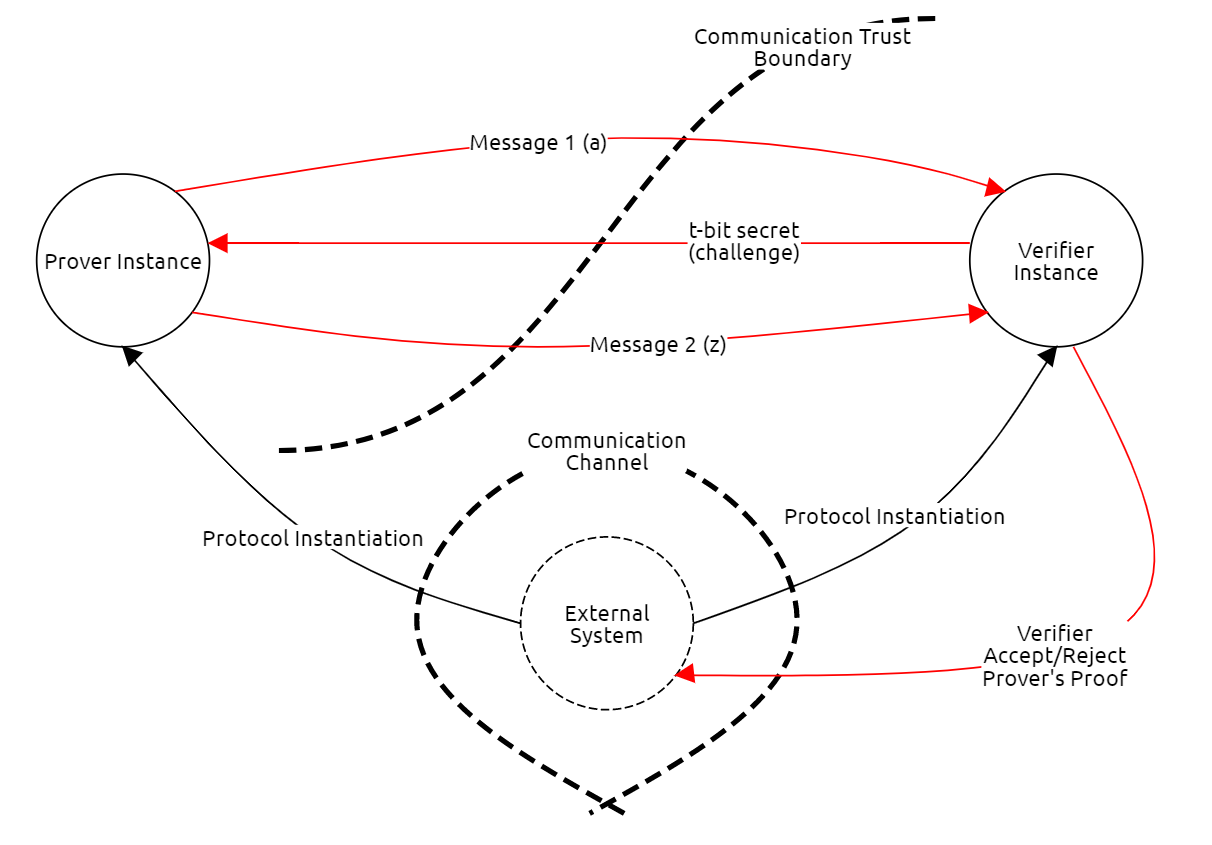
\includegraphics[width=\linewidth]{../assets/threat-model.png}
    \caption{Threat Model Diagram}
    \label{fig:threat_model}
\end{figure}

There should be no known way for adversaries to use the protocol in a way that it is not designed to. For example, under normal circumstances, the verifier should not have rewind access to a prover, this means that we will need to model state within the protocol and ensure that it is used properly (state-machine model). This should be a target of penetration tests. 




\end{document}